\chapter{Parallel implementation}\label{ch:implementation-details}
In this chapter we shall present techniques used to improve the performance of the simulation. We shall present both CPU and GPU parallelization techniques and compare them. The performance will be measured on two machines Computer 1: CPU - Intel(R) Core(TM) i7-3632QM CPU @ 2.20GHz (4 cores, 8 threads), 2 blocks of 4GB SODIMM DDR3 Synchronous 800 MHz RAM and Computer 2: CPU - Intel(R) Core(TM) i7-9700 CPU @ 3.00GHz (8 cores, 8 threads) and 4 blocks of 16GB DDR4 1333 MHz RAM, GPU 1 - NVidia A5000. We shall measure two scenarios - laminar and turbulent flow. Both scenarios will be tested with the following mesh on both machines.

\begin{table}[H]
\centering
\begin{tabular}{|c|r|r|}
\hline
\multicolumn{1}{|l|}{} & \multicolumn{1}{c|}{Mesh} \\ \hline
Elements               & 305854                      \\ \hline
Velocity Nodes         & 613458                      \\ \hline
Pressure Nodes         & 153802                      \\ \hline
\end{tabular}
\end{table}

Let us first sum up the problem and the algorithm used to solve it. We are looking for an approximate solution to the Navier-Stokes equations for a laminar (\cref{eq:laminar_differential_form_recap}) and a turbulent(\cref{eq:turbulent_differential_form_recap}) flow.
\begin{equation}\label{eq:laminar_differential_form_recap}
\begin{aligned}
  &\frac{\partial\mathbf{u}}{\partial t} + \mathbf{u} \cdot \nabla\mathbf{u} = -\nabla p + \nu\Delta\mathbf{u}, &&\left(\mathbf{x}, t\right) \in \Omega \times J \\
  &\nabla \cdot \mathbf{u} = 0, &&\left(\mathbf{x}, t\right) \in \Omega \times J \\
  &\mathbf{u} = 0, &&\left(\mathbf{x}, t\right) \in \left(\Gamma_1 \cup \Gamma_3 \cup \Gamma_5\right) \times J \\
  &\mathbf{u} = \left(\frac{1.2y\left(0.41 - y\right)}{0.41^2}, 0\right), &&\left(\mathbf{x}, t\right) \in \Gamma_4 \times J \\
  &\nu\frac{\partial\mathbf{u}}{\partial\mathbf{n}} - p\mathbf{n} = 0, &&\left(\mathbf{x}, t\right) \in \Gamma_2 \times J \\
\end{aligned}
\end{equation}

\begin{equation}\label{eq:turbulent_differential_form_recap}
\begin{aligned}
  &\frac{\partial\mathbf{u}}{\partial t} + \mathbf{u} \cdot \nabla\mathbf{u} = -\nabla p + \nu\Delta\mathbf{u}, &&\left(\mathbf{x}, t\right) \in \Omega \times J \\
  &\nabla \cdot \mathbf{u} = 0, &&\left(\mathbf{x}, t\right) \in \Omega \times J \\
  &\mathbf{u} = 0, &&\left(\mathbf{x}, t\right) \in \left(\Gamma_1 \cup \Gamma_3 \cup \Gamma_5\right) \times J \\
  &\mathbf{u} = \left(\frac{6y(0.41-y)}{0.41^2}, 0\right), &&\left(\mathbf{x}, t\right) \in \Gamma_4 \times J \\
  &\nu\frac{\partial\mathbf{u}}{\partial\mathbf{n}} - p\mathbf{n} = 0, &&\left(\mathbf{x}, t\right) \in \Gamma_2 \times J \\
\end{aligned}
\end{equation}

To do so at each time step we apply \crefrange{eq:adv-diff-split-advect}{eq:adv-diff-split-velicity-mass}:

\begin{align}
	&\mathbf{Q^A} = advect(KDTree, \mathbf{Q^{i}}, \Delta t) \label{eq:adv-diff-split-advect}\\
		&\left(\begin{bmatrix}
		\mathbf{M} & 0 \\
		0 & \mathbf{M}
	\end{bmatrix} + \nu\Delta t\begin{bmatrix}
		\mathbf{K} & 0 \\
		0 & \mathbf{K}
	\end{bmatrix}\right)\begin{bmatrix}
		\vecf{Q^{B}_1} \\
		\vecf{Q^{B}_2}
	\end{bmatrix} = \begin{bmatrix}
		\mathbf{M} & 0 \\
		0 & \mathbf{M}
	\end{bmatrix}\begin{bmatrix}
		\vecf{Q^{A}_1} \\
		\vecf{Q^{A}_2}
	\end{bmatrix} \label{eq:adv-diff-split-diffuse}\\
	&\mathbf{K_p}\vecf{P}^i = -\frac{1}{\Delta t} \begin{bmatrix}
		\mathbf{B_1} & \mathbf{B_2}
	\end{bmatrix} \begin{bmatrix}
		\vecf{Q^{B}_1} \\
		\vecf{Q^{B}_2}
	\end{bmatrix} \label{eq:adv-diff-split-pressure}\\
	&\begin{bmatrix}
		\mathbf{M} & 0 \\
		0 & \mathbf{M}
	\end{bmatrix} \begin{bmatrix}
		\vecf{Q^{i+1}_1} \\
		\vecf{Q^{i+1}_2}
	\end{bmatrix} =	\begin{bmatrix}
		\mathbf{M} & 0 \\
		0 & \mathbf{M}
	\end{bmatrix} \begin{bmatrix}
		\vecf{Q^{B}_1} \\
		\vecf{Q^{B}_2}
	\end{bmatrix} - \Delta t \begin{bmatrix}
		\vecf{B_{p,1}} \\
		\vecf{B_{p,2}}
	\end{bmatrix} \vecf{P}^i \label{eq:adv-diff-split-velicity-mass}
\end{align}
where the method $advect$ is \cref{alg:Semi-Lagrangian-Advection}.

\section{CPU multithreading}
Our end goal is to implement all algorithms on a GPU. However we need a baseline multithreaded CPU algorithm so that we can measure the pros and cons of using GPU for simulations. In this section we shall present the steps which were taken in order to multithread the chosen method on CPU.

We shall measure the time it takes for the algorithm to compute 1s of simulation time with time step 0.01 i.e. 100 time steps. The baseline for the measurements is the single threaded algorithm. \crefrange{tab:computer1-laminar-baseline}{tab:computer2-turbulent-baseline} present the time spent in each step of the algorithm (\cref{eq:adv-diff-split-advect} - Step 1, \cref{eq:adv-diff-split-diffuse} - Step 2, \cref{eq:adv-diff-split-pressure} - Step 3 and \cref{eq:adv-diff-split-velicity-mass} - Step 4 and the assembling of the corresponding matrices). The measurement is done using C++ timers (std::chrono::steady\_clock) placed at the beginning and ending of each function. The data for executing the algorithm is gathered over 11 sequential runs of the algorithm on Computer 1 and Computer 2 for the given mesh.
\begin{table}[H]
\centering
\begin{tabular}{|c|c|c|c|c|c|c|c|}
\hline
\multirow{3}{*}{} & \multicolumn{7}{c|}{Computer 1}                                                                                                                                       
\\ \cline{2-8}
& Step 1 & Step 2 & Step 3 & Step 4 & \begin{tabular}[c]{@{}c@{}}CG \\ (Total)\end{tabular} & \begin{tabular}[c]{@{}c@{}}Matrix\\ Assembling\end{tabular} & \begin{tabular}[c]{@{}c@{}}Total \\ Time\end{tabular} \\ \hline
\begin{tabular}[c]{{@{{}}c@{{}}}}Mean \\ Time\end{tabular}  & 79.75s & 138.33s & 505.50s & 44.47s & 688.30s & 20.80s & 794.82s\\ \hline SD & 0.64s&3.83s&3.62s&1.30s&8.76s&0.38s&10.01s\\ \hline Median & 80.20s&141.05s&508.06s&45.39s&694.50s&21.07s&801.89s\\ \hline Min & 79.30s&135.62s&502.94s&43.55s&682.11s&20.54s&787.74s\\ \hline Max & 80.20s&141.05s&508.06s&45.39s&694.50s&21.07s&801.89s\\ \hline
\end{tabular}
\caption{Execution time on 1 thread of Computer 1 for solving for laminar flow via \crefrange{eq:adv-diff-split-advect}{eq:adv-diff-split-velicity-mass} over the given mesh with $\Delta t = 0.01$ and Conjugate Gradient method used for solving the linear system.}\label{tab:computer1-laminar-baseline}
\end{table}

\begin{table}[H]
\centering
\begin{tabular}{|c|c|c|c|c|c|c|c|}
\hline
\multirow{3}{*}{} & \multicolumn{7}{c|}{Computer 2}                                                                                                                                       
\\ \cline{2-8}
& Step 1 & Step 2 & Step 3 & Step 4 & \begin{tabular}[c]{@{}c@{}}CG \\ (Total)\end{tabular} & \begin{tabular}[c]{@{}c@{}}Matrix\\ Assembling\end{tabular} & \begin{tabular}[c]{@{}c@{}}Total \\ Time\end{tabular} \\ \hline
\begin{tabular}[c]{{@{{}}c@{{}}}}Mean \\ Time\end{tabular}  & 60.32s & 101.12s & 398.50s & 30.31s & 529.93s & 11.82s & 605.48s\\ \hline SD & 0.15s&0.57s&1.85s&0.05s&2.14s&0.04s&2.27s\\ \hline Median & 60.31s&100.96s&398.29s&30.33s&529.86s&11.84s&605.45s\\ \hline Min & 60.03s&100.56s&395.98s&30.19s&526.75s&11.76s&602.09s\\ \hline Max & 60.54s&102.54s&402.81s&30.37s&534.01s&11.87s&609.62s\\ \hline
\end{tabular}
\caption{Execution time on 1 thread of Computer 2 for solving for laminar flow via \crefrange{eq:adv-diff-split-advect}{eq:adv-diff-split-velicity-mass} over the given mesh with $\Delta t = 0.01$ and Conjugate Gradient method used for solving the linear system.}\label{tab:computer2-laminar-baseline}
\end{table}


%%%%%%%%%%%%%%%%%%%%%%%%%%%%%%%%%%%%%%%%%%%%%%%%%%%%%%%%%%%%%%%%%%%%%%%%%%
%%%%%%%%%%%%%%%%%%%%%%%%%%% TURBULENT %%%%%%%%%%%%%%%%%%%%%%%%%%%%%%%%%%%%
%%%%%%%%%%%%%%%%%%%%%%%%%%%%%%%%%%%%%%%%%%%%%%%%%%%%%%%%%%%%%%%%%%%%%%%%%%
\begin{table}[H]
\centering
\begin{tabular}{|c|c|c|c|c|c|c|c|}
\hline
\multirow{3}{*}{} & \multicolumn{7}{c|}{Computer 1}                                                                                                                                       
\\ \cline{2-8}
& Step 1 & Step 2 & Step 3 & Step 4 & \begin{tabular}[c]{@{}c@{}}CG \\ (Total)\end{tabular} & \begin{tabular}[c]{@{}c@{}}Matrix\\ Assembling\end{tabular} & \begin{tabular}[c]{@{}c@{}}Total \\ Time\end{tabular} \\ \hline
\begin{tabular}[c]{{@{{}}c@{{}}}}Mean \\ Time\end{tabular}  & 80.35s & 196.81s & 597.43s & 55.31s & 849.54s & 20.45s & 956.29s\\ \hline SD & 0.83s&5.57s&3.18s&0.77s&9.52s&0.08s&10.45s\\ \hline Median & 80.94s&200.74s&599.68s&55.86s&856.28s&20.51s&963.68s\\ \hline Min & 79.76s&192.87s&595.18s&54.76s&842.81s&20.40s&948.90s\\ \hline Max & 80.94s&200.74s&599.68s&55.86s&856.28s&20.51s&963.68s\\ \hline
\end{tabular}
\caption{Execution time on 1 thread of Computer 1 for solving for turbulent flow via \crefrange{eq:adv-diff-split-advect}{eq:adv-diff-split-velicity-mass} over the given mesh with $\Delta t = 0.01$ and Conjugate Gradient method used for solving the linear system.}\label{tab:computer1-turbulent-baseline}
\end{table}

\begin{table}[H]
\centering
\begin{tabular}{|c|c|c|c|c|c|c|c|}
\hline
\multirow{3}{*}{} & \multicolumn{7}{c|}{Computer 2}                                                                                                                                       
\\ \cline{2-8}
& Step 1 & Step 2 & Step 3 & Step 4 & \begin{tabular}[c]{@{}c@{}}CG \\ (Total)\end{tabular} & \begin{tabular}[c]{@{}c@{}}Matrix\\ Assembling\end{tabular} & \begin{tabular}[c]{@{}c@{}}Total \\ Time\end{tabular} \\ \hline
\begin{tabular}[c]{{@{{}}c@{{}}}}Mean \\ Time\end{tabular}  & 61.22s & 143.49s & 541.06s & 37.69s & 722.23s & 11.90s & 798.78s\\ \hline SD & 0.31s&0.77s&3.23s&0.17s&3.97s&0.12s&4.25s\\ \hline Median & 61.35s&143.62s&542.91s&37.73s&724.74s&11.89s&801.48s\\ \hline Min & 60.74s&142.42s&535.43s&37.39s&716.07s&11.75s&792.43s\\ \hline Max & 61.71s&144.89s&544.70s&38.03s&727.36s&12.17s&804.32s\\ \hline
\end{tabular}
\caption{Execution time on 1 thread of Computer 2 for solving for turbulent flow via \crefrange{eq:adv-diff-split-advect}{eq:adv-diff-split-velicity-mass} over the given mesh with $\Delta t = 0.01$ and Conjugate Gradient method used for solving the linear system.}\label{tab:computer2-turbulent-baseline}
\end{table}

Although these two examples are not comprehensive and more tests with different scenarios must be made, they give us a few hints about the behaviour of the program. The bulk of the time is spent in the Conjugate Gradient method, with \cref{eq:adv-diff-split-pressure} being the most computationally expensive. The matrix used when solving the Pressure Poisson equation is smaller than the other matrices, thus it is logical to assume that the method needs more iterations in order to converge. It looks like turbulent flows need more iterations of the Conjugate Gradient method, most likely because the flow is less ``predictable''.

\subsection{Building the FEM matrices}
The case we are studying is restricted to geometry which is not changing with time. In this case the matrices used by the FEM are constant and are built once at the beginning of the solution. The problem with assembling FEM matrices in a multithreaded fashion is similar to computing IC0 preconditioners in multithreaded fashion. It depends on the topology of the mesh. Usually graph coloring algorithms are used in order to find which elements will not interfere with one another and fill in the matrix for them in parallel. This technique is also not trivial. Given the fact that the matrices are assembled once and that the assembling takes a small fraction of time, a simpler technique was used - each matrix was computed on a separate thread. Since there are 5 matrices we need 5 threads. This way the assembling of the matrices takes time equal to the time for the most expensive matrix (given that we have 5 or more threads at our disposal). This is a simplistic technique but it gives satisfactory results. Implementing graph coloring is left for further research.

\subsection{Multithreading the advection phase}\label{sec:mt-advection}
\subsubsection{A brief introduction to the KD Tree data structure}
KD Trees are binary trees which are very commonly used in ray tracing for acceleration of ray-mesh intersections \cite{pbrt} and in artificial intelligence for solving the k nearest neighbours (KNN) problem \cite{knn-ai}. Originally they were used to handle large sets of points in a k dimensional space (thus the name KD Tree), but they are trivially extendable to handle different kinds of geometrical objects e.g. k dimensional spheres, triangles in 2D and 3D. We will focus on building KD Tree for the 2D space, which will be used to accelerate two types of queries: find in which triangle of a FEM mesh a given point lies and find the nearest node of our FEM mesh to a given point in space.

We begin with a procedure for building a KD Tree (see \cref{alg:build-kd}). Each non-leaf node is a tuple of the form (Axis, Splitting Point, Left Child, Right Child), leaf nodes contain a list of elements assigned to them during the construction of the tree. Initially we begin with a root node, an axis aligned bounding box for the FEM mesh and a set of triangles representing the FEM mesh. The axis aligned bounding boxes are represented with their lower left and upper right vertices. At each point we choose an axis and a point along the axis. Then we imagine that there is a line orthogonal to the axis and containing the selected point. All elements on one side of the line are assigned to one of the children. The other elements (which are on the other side of the line) are assigned to the other (see \cref{fig:kd-build}). Should a triangle lie in both subspaces defined by the line it is assigned to both children. This continues recursively until the count of the triangles in a node gets below some cutoff value or the maximal allowed depth is reached.

\begin{figure}
  \centering
  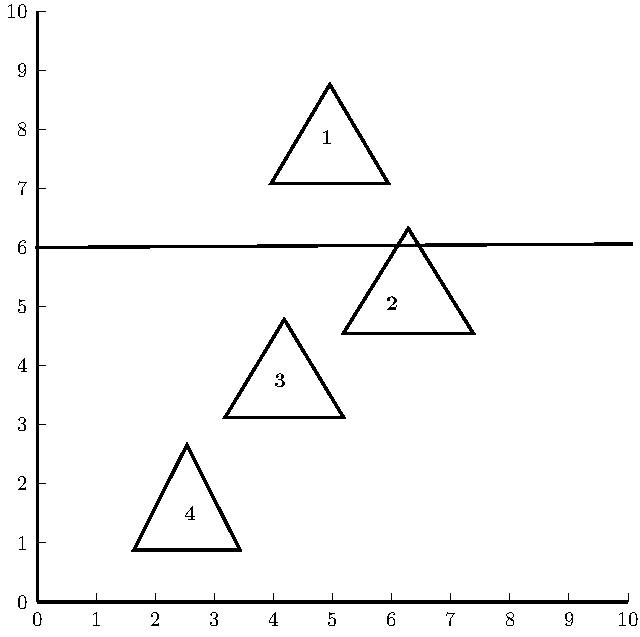
\includegraphics[width=0.5\textwidth]{Figures/kd-example.pdf}
  \caption{The chosen axis is the $y$ axis and the splitting point is 6. A line passing through (0, 6) and orthogonal to the $y$ axis separates the space into two subspaces. Triangles 1 and 2 will be in the right subtree, triangles 2, 3, 4 will be in the left subtree.}\label{fig:kd-build}
\end{figure}

\begin{algorithm}[H]
\centering
\caption{Build KD Tree}\label{alg:build-kd}
\begin{algorithmic}[1]
		\Procedure{BuildKD}{$node, triangles, AABB, depth$}
			\If{$count(triangles) \leq leafSize \lor depth \geq maxDepth$}
				\State \Return makeLeaf(triangles)
			\EndIf
			\State $axis \gets chooseAxis()$
			\State $split \gets chooseSplitPoint()$
			\State $node.axis \gets axis$
			\State $node.split \gets split$
			\State $splitBox(AABB, axis, split, leftAABB, rightAABB)$
			\State $leftTriangles \gets \{\}$
			\State $rightTriangles \gets \{\}$
			\ForAll{t $\in$ triangles}
				\If{$t.A[axis] \leq split \lor t.B[axis] \leq split \lor t.C[axis] \leq split$}
					\State insert(leftTriangles, t)
				\EndIf
				\If{$t.A[axis] \geq split \lor t.B[axis] \geq split \lor t.C[axis] \geq split$}
					\State insert(rightTriangles, t)
				\EndIf
			\EndFor
			\State $root.left \gets BuildKD(leftTriangles, leftAABB, depth + 1)$
			\State $root.right \gets BuildKD(rightTriangles, rightAABB, depth + 1)$
			\State \Return root
		\EndProcedure
\end{algorithmic}
\end{algorithm}

Next we present a procedure (see \cref{alg:get-triangle}) which finds which triangle (if any) contains a point. It is a straightforward task, we just need to traverse the tree. If the given point lies in the left bounding box we follow the left child, otherwise, we follow the right. When we reach a leaf, we need to iterate all triangles in it to see if the point lies in any of them. It is obvious that, given a balanced tree, the complexity of this task is $O(\log{m})$ where m is the number of triangles in the tree.

\begin{algorithm}[H]
\centering
\caption{Find in which triangle a point lies}\label{alg:get-triangle}
\begin{algorithmic}[1]
	\Procedure{FindTriangle}{$node, point$}
		\If{isLeaf(node)}
			\ForAll{$triangle \in node.triangles$}
				\If{$point \in triangle$}
					\State \Return triangle
				\EndIf
			\EndFor
			\Return null
		\EndIf
		\If{$point[node.axis] \leq node.split$}
			\State \Return FindTriangle(node.left, point)
		\Else
			\State \Return FindTriangle(node.right, point)
		\EndIf
	\EndProcedure
\end{algorithmic}
\end{algorithm}

Finding the nearest neighbour is a bit more complex than checking in which triangle a point lies, but the idea is basically the same. The problem is that the nearest mesh point could lie on the opposing side of the splitting axis and thus it is not enough to traverse the tree until reaching the first leaf (see \cref{fig:nearest-neighbour}). To find the nearest point we start traversing the tree recursively, but we need to visit both children of a given node. There is a common optimization which significantly improves the performance for the average case. Let us call the child whose subspace contains the point from the query the near child and the other child the far child. When traversing the tree we must always go to the near child and traverse down to the far child only when distance to the separating plane is less than the distance between the query point and the current nearest neighbour, \cref{alg:nearest-neighbour} presents this idea. Let us note that, although this improves the average case complexity to $O(\log{n})$ where n is the number of points, the worst case, however, is still $O(n)$.

\begin{figure}[H]
  \centering
  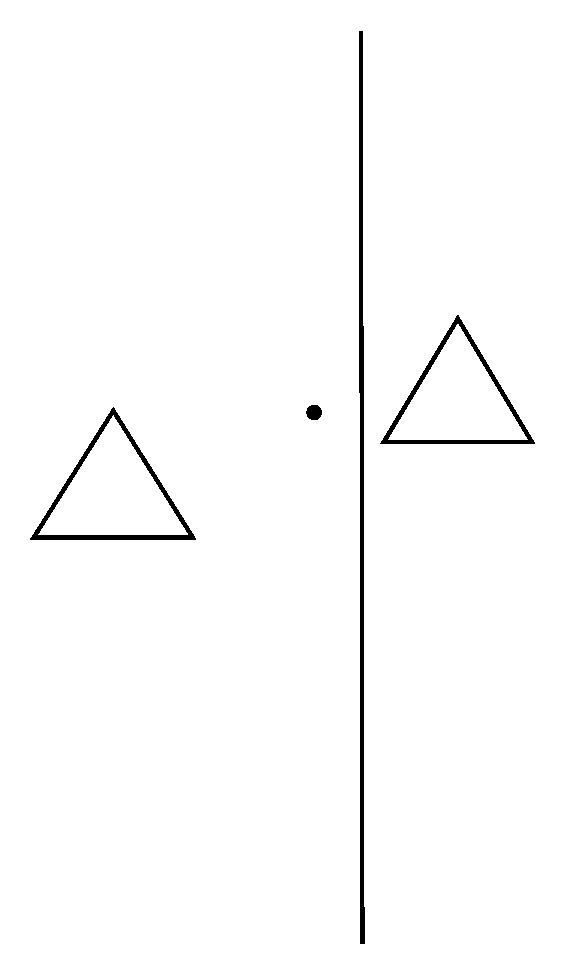
\includegraphics[scale=0.4]{Figures/nearest-neighbour.pdf}
  \caption{The nearest point of the mesh does not always lie in the same subspace, with respect to the separating axis, as the input point.}
  \label{fig:nearest-neighbour}
\end{figure}

\begin{algorithm}[H]
\centering
\caption{Find the nearest point from a FEM mesh to a given point in space}\label{alg:nearest-neighbour}
\begin{algorithmic}[1]
	\Procedure{NearestNeighbour}{$node, point, currentResult$}
		\If{isLeaf(node)}
			\State $result \gets currentResult$
			\ForAll{$triangle \in node.triangles$}
				\ForAll{$node \in triangle$}
					\If{$distance(node, point) < result.distance$}
						\State $result.distance \gets distance(node, point)$
						\State $result.point \gets node$
					\EndIf
				\EndFor
			\EndFor
			\State \Return result
		\EndIf
		\State$near \gets node.left$
		\State$far  \gets node.right$
		\If{$point[node.axis] > node.split$}
			\State swap(near, far)
		\EndIf
		\State $result \gets NearestNeighbour(near, point, currentResult)$
		\If{$result.distance > abs(point[node.axis] - node.split)$}
			\State $result \gets NearestNeighbour(far, point, result)$
		\EndIf
		\State \Return result
	\EndProcedure
\end{algorithmic}
\end{algorithm}

\subsubsection{KD Tree implementation details}
Before discussing the multithreading part we shall give some implementation details about the KD Tree and a commentary on how it should be improved. The tree is built in a recursive top-down fashion. It is stored in a linear array, the root is stored at index 0. If a node has index $i$ in the array its left child is always stored at index $i+1$, while its right child is stored at some other index which is not important. In our case for a given node we first build its left subtree and then the right subtree. Thus the index of the right child is the first free index after the last node of the left subtree. Such ordering is cache friendly, because when we reach a node its left child will always be on the same cache line. The maximum allowed depth is 29 and in case a node has less than 16 triangles in it, it is made a leaf. The cutoff value of 16 does not have any specific reasoning behind it, different values were tested and there were no significant changes in runtime. The most important part of building a KD tree for this case is to make it as balanced as possible. At each step a splitting point along the splitting axis must be chosen such that the difference between the number of triangles on both of its sides is as small as possible. There are two -- questions how to choose the axis and how to choose the point. We select the axes in a round-robin fashion. Our strategy for choosing a split point is to split the bounding box of the parent node in the center, along the splitting axis, subdividing it into equal sized bounding boxes for each child. This strategy is rather simplistic and does not work well. For small meshes such as the given mesh it is tolerable and the run time is still dominated by the CG method, however should the given mesh become, say, 2 times larger  the runtime increases unproportionally, making the method borderline unusable. A better approach should be implemented. The simplest approach is to use the Quickselect algorithm \cite{introduction-to-algorithms} in order to find the median of the points in the current tree and use it as a splitting point when subdividing into subtrees. The algorithm has best and average case complexity of $O(n)$ where $n$ is the number of points, but worst case of $O(n^2)$. It was implemented and it significantly improved the tree traversal performance. However this increased the time needed to build the tree by a substantial amount. This happens because the algorithm must be executed for each node. Thus making it a viable choice when the simulation has a large amount of steps. Another option is to use the PICK algorithm \cite{pick}, it is a well known algorithm for finding the median of an array in deterministic $O(n)$ time. We have not tried to implement it. On one hand it is not trivial to implement on the other hand, although, it has asymptotically linear time, the constant (which is implied by the notation) is known to be large, thus making it slower than Quickselect with random pivot selection, until the data set becomes large enough. Due to this reason we think that it falls out of the scope of the current work. It would be interesting to implement it, however. Another approach worth trying is described in \cite{Balanced-KD-Tree}.

\subsubsection{Splitting the work between threads}
As it was already mentioned the semi-Lagrangian algorithm is trivial to parallelize. We shall use simple fork-join technique to do so. It is obvious that each quantity at each vertex (in our case only the velocity is advected, but  in general there can be other quantities such as temperature, concentration, etc.) can be advected on its own without interacting with the other advected quantities and other mesh vertices. Thus we shall split all velocity nodes into groups and each group should be scheduled to a separate CPU thread. For the implementation we use the Thread Building Blocks (TBB) multithreading library provided by Intel. It does the job of spawning threads and distributing work between them, while we shall only pass the function which will be executed on each thread. Next we present how this scales with multiple threads see( \crefrange{fig:advection_speedup_graph_laminar}{fig:advection_speedup_graph_turbulent}). For more detailed view refer to \cref{ch:stastical-data}

\subsubsection{Speedup results}
\begin{figure}[H]
  \centering
  \begin{subfigure}[b]{0.49\textwidth}
      \centering
      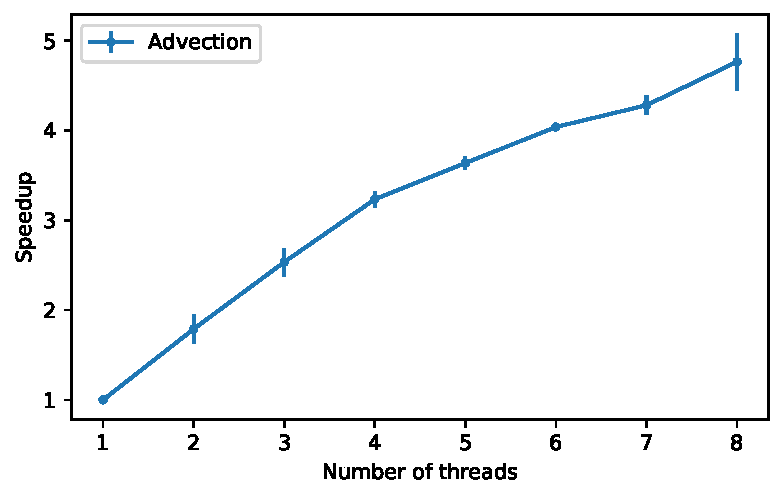
\includegraphics[width=\textwidth]{Figures/LaminarAdvectionSpeedUpC1.pdf}
      \caption{Computer 1}
  \end{subfigure}
  \begin{subfigure}[b]{0.49\textwidth}
      \centering
      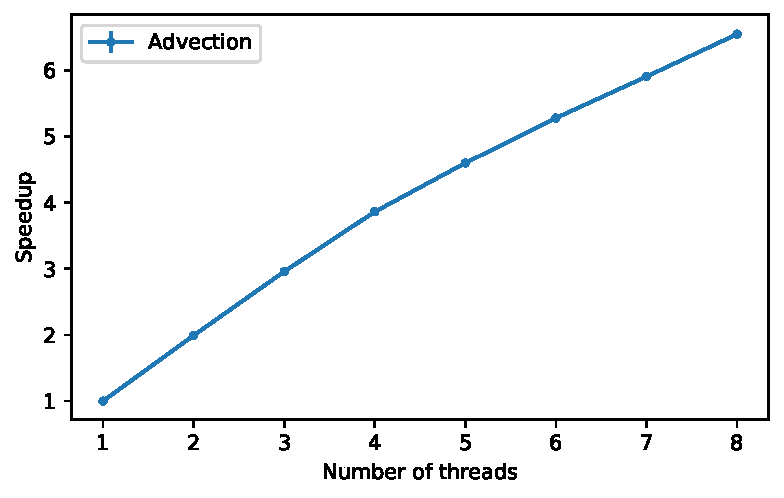
\includegraphics[width=\textwidth]{Figures/LaminarAdvectionSpeedUpC2.pdf}
      \caption{Computer 2}
  \end{subfigure}
\caption{Scaling of \cref{eq:adv-diff-split-advect} solved via semi-Lagrangian method with $\Delta t = 0.01$ over the given mesh for laminar flow. Vertical bars represent 2 times the standard deviation of the measured speedup.}\label{fig:advection_speedup_graph_laminar}
\end{figure}

\begin{figure}[H]
  \centering
  \begin{subfigure}[b]{0.49\textwidth}
      \centering
      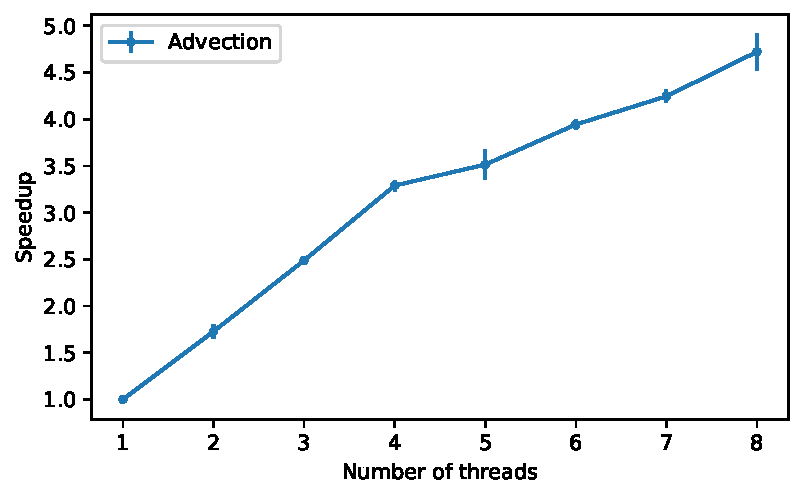
\includegraphics[width=\textwidth]{Figures/TurbulentAdvectionSpeedUpC1.pdf}
      \caption{Computer 1}
  \end{subfigure}
  \begin{subfigure}[b]{0.49\textwidth}
      \centering
      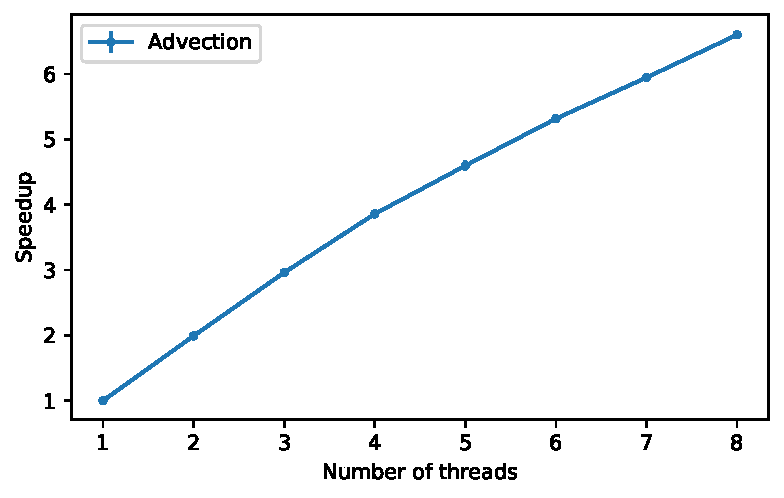
\includegraphics[width=\textwidth]{Figures/TurbulentAdvectionSpeedUpC2.pdf}
      \caption{Computer 2}
  \end{subfigure}
\caption{Scaling of \cref{eq:adv-diff-split-advect} solved via semi-Lagrangian method with $\Delta t = 0.01$ over the given mesh for turbulent flow. Vertical bars represent 2 times the standard deviation of the measured speedup.}\label{fig:advection_speedup_graph_turbulent}
\end{figure}

From the provided data we can see that the algorithm scales with increasing the number of threads. The standard deviation is low, meaning that the runtime does not fluctuate. One thing which should be noted is that according to the data, the achieved speedup for Computer 1 drops a bit when the mark of 5 threads is reached. After that the speedup still increases when the number of threads increases, but it is further from the expected one. This phenomenon is due to Intel Hyper-Threading technology. Computer 1 is a quad core computer. This means that in theory only 4 tasks can be executed in parallel, thus the speedup is much better in the range [2;4] threads. However modern CPUs have very complicated architecture. One CPU core contains multiple arithmetic units, pipelines, cache and branch predictors, etc. It often happens that one thread cannot fully utilize the CPU. Imagine the simplest case possible, the thread does only integer operations. In this case all floating point arithmetic units are idle. Intel Hyper-Threading technology addresses this issue, by presenting each physical core as 2 logical cores. This way through clever task scheduling the CPU can be utilized better. This technique has its limitations and it is obvious that using threads more than the number of cores does not mean that the performance should double. On the other hand Computer 2 has 8 core processor and does not support Hyper-Threading. We can see that the algorithm, indeed, continues scaling in an almost linear fashion even beyond the 4 threads mark.

\subsection{Conjugate Gradient}
Contrary to the advection, Conjugate Gradient cannot be multithreaded as a whole. However we can multithread each step of it: the matrix vector product, the vector additions and the dot product. All of these are trivially parallelizable on their own. TBB was used for this part as well. For the vector matrix product the matrix is split into blocks, each block containing some set of rows. Thus each CPU thread gets to compute all dot products of the rows in its block of the matrix and the vector which multiplies the matrix. For the vector additions we use a similar technique, the vectors are split in blocks and each CPU thread gets to add the parts of the two vectors in its block. For the dot product the built-in tbb::parallel\_deterministic\_reduce operation is used, it also uses the same idea, and splits the vectors into blocks, then each CPU thread computes the dot product of the subvectors in its block, this leaves us with an array $a_1, a_2, ... a_n$ of the computed (sub) dot products, which must be added together in order to compute the final result. What tbb::parallel\_deterministic\_reduce does is to provide specific order to all additions so that the result of the dot product is always deterministic. The downside of it is that TBB cannot dynamically split the workload and the sizes of each block must be defined by the programmer. We have empirically chosen blocks of size 8192. As we mentioned the Conjugate Gradient cannot be multithreaded as a whole, and the reason is the dot product which acts as a barrier between the separate phases of the algorithm. Next in \cref{fig:laminar-scaling} and \cref{fig:turbulent-scaling} we provide graphics and tables showing how the algorithm scales to multi-core systems and a commentary on the achieved results.

%%%%%%%%%%%%%%%%%%%%%%%%%%%%%%%%%%%%%%%%%%%%%%%%%%%%%%%%%%%
%%%%%%%%%%%%%%%%%%%%%% LAMINAR %%%%%%%%%%%%%%%%%%%%%%%%%%%%
%%%%%%%%%%%%%%%%%%%%%%%%%%%%%%%%%%%%%%%%%%%%%%%%%%%%%%%%%%%

\begin{figure}[H]
  \centering
  \begin{subfigure}[b]{0.8\textwidth}
      \centering
      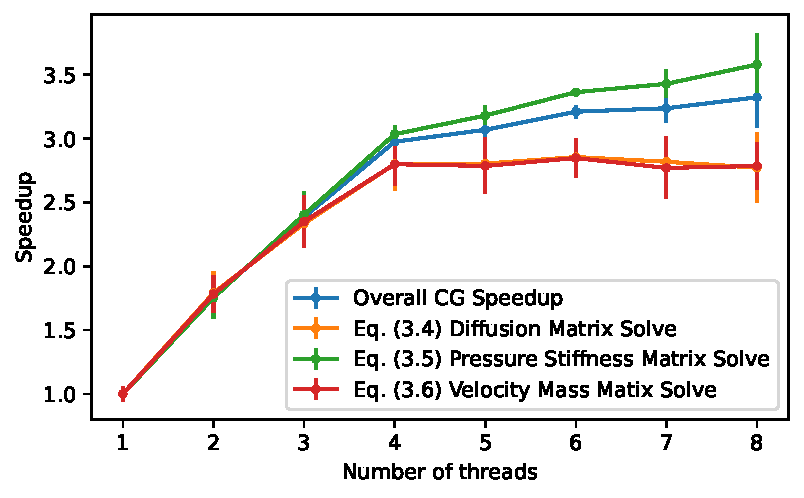
\includegraphics[width=\textwidth]{Figures/LaminarCGSpeedUpC1.pdf}
      \caption{Computer 1}
  \end{subfigure}
\end{figure}
\begin{figure}[H]
	\centering
  \ContinuedFloat
  \begin{subfigure}[b]{0.8\textwidth}
      \centering
      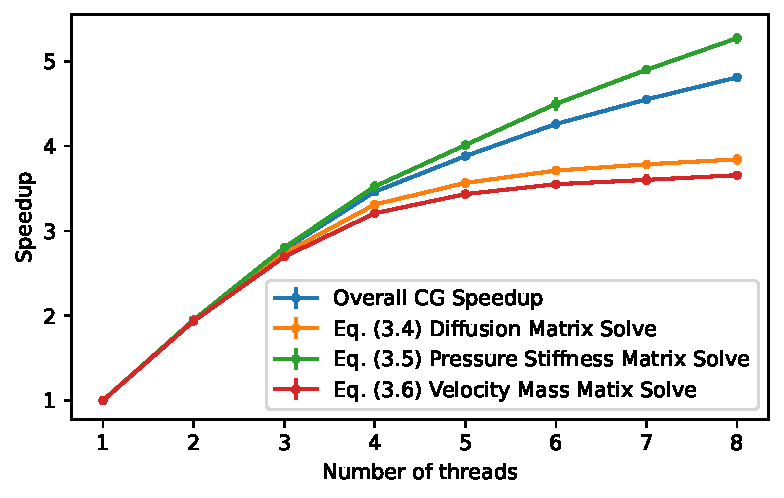
\includegraphics[width=\textwidth]{Figures/LaminarCGSpeedUpC2.pdf}
      \caption{Computer 2}
  \end{subfigure}\caption{Scaling of \crefrange{eq:adv-diff-split-pressure}{eq:adv-diff-split-velicity-mass} solved via Conjugate Gradient method with tolerance of $10^{-8}$ applied over the given mesh for laminar flow. Vertical bars represent 2 times the standard deviation of the measured speedup.}
  \label{fig:laminar-scaling}
\end{figure}


%%%%%%%%%%%%%%%%%%%%%%%%%%%%%%%%%%%%%%%%%%%%%%%%%%%%%%%
%%%%%%%%%%%%%%%%%%%%%% TURBULENT %%%%%%%%%%%%%%%%%%%%%%
%%%%%%%%%%%%%%%%%%%%%%%%%%%%%%%%%%%%%%%%%%%%%%%%%%%%%%%
\begin{figure}[H]
  \centering
  \begin{subfigure}[b]{0.8\textwidth}
      \centering
      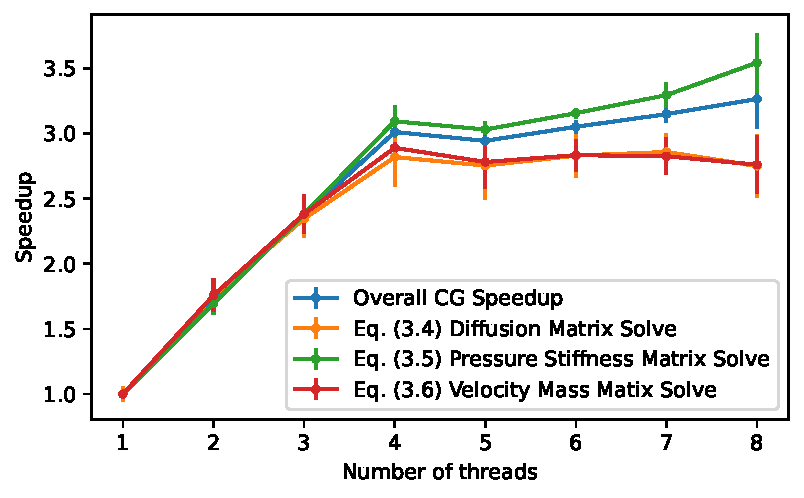
\includegraphics[width=\textwidth]{Figures/TurbulentCGSpeedUpC1.pdf}
      \caption{Computer 1}
  \end{subfigure}
\end{figure}
\begin{figure}[H]
	\centering
  \ContinuedFloat
  \begin{subfigure}[b]{0.8\textwidth}
      \centering
      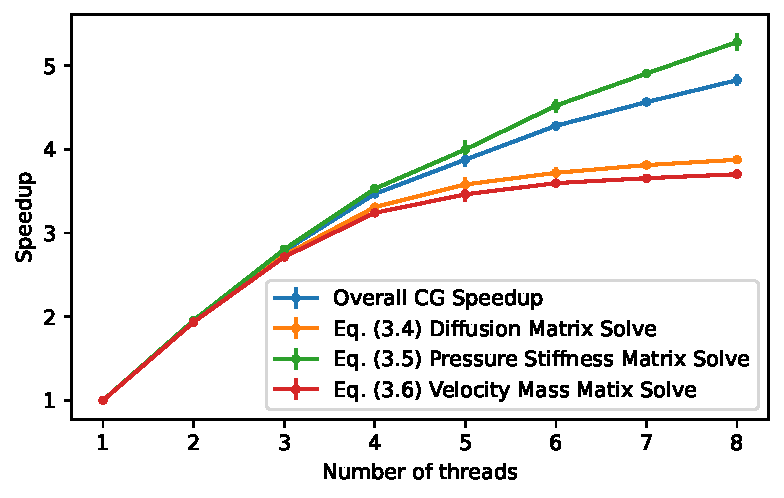
\includegraphics[width=\textwidth]{Figures/TurbulentCGSpeedUpC2.pdf}
      \caption{Computer 2}
  \end{subfigure}\caption{Scaling of \crefrange{eq:adv-diff-split-pressure}{eq:adv-diff-split-velicity-mass} solved via Conjugate Gradient method with tolerance of $10^{-8}$ applied over the given mesh for turbulent flow. Vertical bars represent 2 times the standard deviation of the measured speedup.}
  \label{fig:turbulent-scaling}
\end{figure}

The plots show how each of \crefrange{eq:adv-diff-split-pressure}{eq:adv-diff-split-velicity-mass} scale and how the method scales overall\footnote{Note, the overall scaling is not the mean scaling of \crefrange{eq:adv-diff-split-pressure}{eq:adv-diff-split-velicity-mass}. It is the total time spent in the CG method on one thread divided by the total time spent in the CG method on multiple threads. It behaves more like a weighted average of \crefrange{eq:adv-diff-split-pressure}{eq:adv-diff-split-velicity-mass}. The equations which are more time consuming have a higher weight.}. From the plots we see that the method scales worse than the advection. Solving \cref{eq:adv-diff-split-velicity-mass} and \cref{eq:adv-diff-split-diffuse} scales up to about 4 cores and then almost stops scaling. The hyperthreading technology does not help much. We see that it improves the average speedup but the standard deviation is so large, hinting that most of the results are just noise. Looking at Computer 2 which has 8 physical cores we see that these equations indeed stop gaining any significant speedup after the 4 core mark.

On the other hand solving the Pressure Poisson equation gained speedup even with hyperthreading. There are two issues here. First, although each step of the CG method is parallelizable, the operations done at each step are simple (adding vectors together or computing dot products). Contemporary CPUs are very good at these things and increasing the core count does not help simply because there is not enough work to do. To make things worse the modern CPUs are so good at simple arithmetics, that they are faster than loading data from the memory. Second problem is concerned with \cref{eq:adv-diff-split-velicity-mass} and \cref{eq:adv-diff-split-diffuse}. They do not scale because CG does a small amount of iterations with them, compared to the number of iterations done while solving the Pressure Poisson system, \cref{tab:CG-iterations} shows the number of iterations done by the CG method for each equation.

One thing to note is that our implementation of the CG does not take advantage of superscalar instructions (SSE4.2, AVX, AVX2)  \cite{x86-manual}. The theoretical speed which they can provide is up to 4 (SEE4.2), 8 (AVX), 16 (AVX2). It is highly unlikely to reach the maximal theoretical speedup, but we are optimistic that they will provide considerable speedup. Implementing the CG method using superscalar instructions is left for further research.

The conclusion we can draw from this experiment is that the CG method scales to multiple processors only if there is enough data to saturate the CPU. There is always a point at which throwing more cores at the problem will not improve the performance. Thus it is better to aim at a CPU with higher clock rate.

\subsubsection{Preconditioning}

Given CG methods require a lot of computational time, we have tried to reduce the number of iterations done by it and therefore we have hoped that the run time would also be reduced. For that purpose we have decided to implement a preconditioned CG method. Since all matrices are symmetric and positive definite, the logical choice was to implement zero fill-in Incomplete Cholesky Preconditioner (IC0). As we can see from \cref{tab:CG-iterations} the iterations done by the preconditioned method were significantly lowered. However we have faced two problems. Our implementation of the factorization is not multithreaded and did take a lot of time. Of course, when the simulation time is increased, this effect will become smaller. Since the matrices involved in solving \cref{eq:adv-diff-split-velicity-mass} and \cref{eq:adv-diff-split-diffuse} are larger than the one involved in Pressure Poisson equation, computing a preconditioner for them takes significantly more time. Given the fact that we spent significantly more time solving the Pressure Poisson system it is justifiable not to build preconditioners for \cref{eq:adv-diff-split-velicity-mass} and \cref{eq:adv-diff-split-diffuse}. The second problem we have encountered is at the application of the preconditioner, which is also single threaded. Although the number of iterations is cut in half the performance was almost the same for single threaded execution (see \crefrange{tab:ic0-timings}{tab:solve-ic0-8-thread}). In order to apply the preconditioner two triangular systems must be solved. Multithreading of such tasks depends on the structure of the mesh and also on the numbering of the nodes and is left for further research (see \cref{ch:further-development}).

Implementing multithreaded computation of IC0 preconditioner and multithreaded application of it is not a trivial task and is left for further research. It's worth noting that the multithreaded properties of the algorithms are limited and highly depend on the structure of the underlying matrices (and on the geometry of the simulation). Usually the recommended preconditioner in a multithreaded environment is the Block Jacobi preconditioner \cite{Bridson}, \cite{saad-sparse}. Further research is needed in order to compare them.

\begin{table}[H]
\centering
\begin{tabular}{|c|c|c|c|}
\hline Differential problem
& \begin{tabular}[c]{@{}c@{}}Total iterations\\ \cref{eq:adv-diff-split-pressure}\end{tabular} & \begin{tabular}[c]{@{}c@{}}Total iterations\\ \cref{eq:adv-diff-split-velicity-mass}\end{tabular} & \begin{tabular}[c]{@{}c@{}}Total iterations\\ \cref{eq:adv-diff-split-diffuse}\end{tabular} \\ \hline
Laminar flow              & 195422 & 2763 & 10370  \\ \hline
Turbulent flow            & 264394 & 3504 & 14820  \\ \hline
Laminar flow (IC0)   &  72353 &  495 &  1855  \\ \hline
Turbulent flow (IC0) &  85047 &  693 &  2693  \\ \hline
\end{tabular}\caption{Total number of iterations done by the CG method with the given mesh after 100 time-steps of \crefrange{eq:adv-diff-split-advect}{eq:adv-diff-split-velicity-mass}  with $\Delta t = 0.01$}\label{tab:CG-iterations}
\end{table}

% ====================================================================================================
% =========================================== COMPUTE IC0 ============================================
% ====================================================================================================

\begin{table}[H]
\centering
\begin{tabular}{|c|c|c|c|c|c|}
\hline
                                                                                   & \begin{tabular}[c]{@{}c@{}}Mean\\ Time\end{tabular} & Median & SD   & \begin{tabular}[c]{@{}c@{}}Min\\ Time\end{tabular} & \begin{tabular}[c]{@{}c@{}}Max\\ Time\end{tabular} \\ \hline
\begin{tabular}[c]{@{}c@{}}Compute IC0 for\\ Pressure Stiffness Matrix\end{tabular} 
& 15.66 & 15.67  & 0.02 & 15.64  & 15.68                                              \\ \hline
\begin{tabular}[c]{@{}c@{}}Compute IC0 for\\ Velocity Mass Matrix\end{tabular} 
& 390.33 & 389.98 & 1.32 & 389.22 & 391.79                                             \\ \hline
\begin{tabular}[c]{@{}c@{}}Compute IC0 for\\ Diffusion Matrix\end{tabular}          
& 380.68 & 379.17 & 4.98 & 376.62  & 386.23                                             \\ \hline
\end{tabular}\caption{Time needed to compute the IC0 preconditioner on a single thread on Computer 2 for all matrices.}\label{tab:ic0-timings}
\end{table}

\begin{table}[H]
\centering
\begin{tabular}{|c|c|c|c|c|c|}
\hline
     & \begin{tabular}[c]{@{}c@{}}Mean\\ Time\end{tabular} & Median & SD   & \begin{tabular}[c]{@{}c@{}}Min\\ Time\end{tabular} & \begin{tabular}[c]{@{}c@{}}Max\\ Time\end{tabular} \\ \hline
Solve \cref{eq:adv-diff-split-pressure} & 393.30 & 393.50 & 0.29 & 393.09 & 393.50 \\ \hline
Solve \cref{eq:adv-diff-split-velicity-mass} & 22.01 & 22.03  & 0.03 & 21.99 & 22.03 \\ \hline
Solve \cref{eq:adv-diff-split-diffuse} & 54.76 & 54.76  & 0.00 & 74.75 & 54.76 \\ \hline
\end{tabular}\caption{Time needed to solve \crefrange{eq:adv-diff-split-pressure}{eq:adv-diff-split-velicity-mass} by PCG with IC0 preconditioner for a laminar flow on a single thread on Computer 2}\label{tab:solve-ic0-1-thread}
\end{table}

\begin{table}[H]
\centering
\begin{tabular}{|c|c|c|c|c|c|}
\hline
     & \begin{tabular}[c]{@{}c@{}}Mean\\ Time\end{tabular} & Median & SD   & \begin{tabular}[c]{@{}c@{}}Min\\ Time\end{tabular} & \begin{tabular}[c]{@{}c@{}}Max\\ Time\end{tabular} \\ \hline
Solve \cref{eq:adv-diff-split-pressure} & 252.75 & 259.95 & 10.19 & 245.54 & 259.95 \\ \hline
Solve \cref{eq:adv-diff-split-velicity-mass} & 15.54 & 15.55  & 0.02 & 15.52 & 15.55 \\ \hline
Solve \cref{eq:adv-diff-split-diffuse} & 37.77 & 37.86 & 0.12 & 37.68 & 37.86 \\ \hline
\end{tabular}\caption{Time needed to solve \crefrange{eq:adv-diff-split-pressure}{eq:adv-diff-split-velicity-mass} by PCG with IC0 preconditioner for a laminar flow on 8 threads on Computer 2. The preconditioner is applied on single thread, however, the other steps of the method (dot product, vector matrix multiplication and vector addition) are computed on 8 threads.}\label{tab:solve-ic0-8-thread}
\end{table}

\subsection{Conclusion}
\begin{itemize}
	\item Building the FEM matrices takes a small amount of time compared to solving the equations. If the geometry is not changing over time, it is acceptable to build all matrices upfront, each matrix can be built on a separate thread.
	\item The semi-Lagrangian approach scales almost linearly with the increase of the CPU cores.
	\item Building KD trees by choosing the midpoint of the splitting axis as a separation point works for small meshes. For large meshes it produces an unbalanced tree which is slow to traverse.
	\item CG method is composed of simple operations. It scales well with the increase of CPU cores only when there are enough operations to saturate the CPU.
	\item IC0 preconditioning reduces significantly the number of iterations needed for the CG method in order to converge.
	\item Single threaded computation and application of IC0 are impractical.
\end{itemize}

\section{GPU Implementation}
Our GPU implementation is written in CUDA, a general purpose language provided by NVidia. Applications written in CUDA can be run only on NVidia GPUs. However GPU architectures do not vary drastically between different vendors, thus the lessons learned from the experiments should be valid for all vendors.
\subsection{A brief introduction to GPU architecture and programming model}
Here we shall present the GPU architecture and introduce the terms which are used later in the research. For detailed explanation refer to the NVidia Programming Guide\footnote{The programming guide is available at \url{https://docs.nvidia.com/cuda/cuda-c-programming-guide/index.html}. This page links to the programming guide for the latest version of the CUDA language}.

GPUs and CPUs have evolved to do different tasks, thus they have different architecture and excel at different problems. Widespread CPUs have relatively small core count, usually between 2 and 16. Only recently companies started producing mainstream CPUs with higher core count with AMDs 64 core Threadripper being one of the mainstream CPUs with highest core count\footnote{The Threadripper has 64 physical cores which can effectively spawn 128 threads}. A single CPU core has a higher clock rate (compared to a single GPU core) and it excels at doing sequential work. CPUs deal with latency (waiting for data to arrive from the RAM, waiting for other instructions to complete, etc.) by having a lot of supplementary hardware, besides the arithmetic units and registers. They have sophisticated memory caching systems (because waiting for data from RAM is slow), prefetching systems which try to predict from which part of the RAM data will be requested and fetch it in advance, branch prediction, instructions are decomposed to even smaller instructions and executed on a pipeline, instructions can be executed out of order and the list goes on and on.

On the other hand NVidia GPUs have higher CUDA core count starting from a few hundred and reaching to a few thousand, depending on the GPU architecture. For example NVidia A5000 card has 8,192 CUDA cores. CUDA cores, however, have lower clock rate, there is no branch prediction, prefetching, out of order execution. We can compare a CUDA core to a single lane in a superscalar CPU. On an NVidia GPU, CUDA cores are distributed among several Streaming Multiprocessors (SM). For example NVidia A5000 has 64 SMs. The streaming multiprocessor is responsible for fetching data and instructions and execution scheduling. Each instruction is executed \textit{simultaneously} by 32 CUDA cores (called a warp)\footnote{Modern NVidia architectures sometimes can divide a warp into 2 half-warps}. When a warp reaches a conditional statement and some of the threads need to take one code path, while others need to take the other code we have thread (execution) divergence. The GPU will execute the first branch, with the threads which enter it, while the others are idle and then the second. Having thread divergence slows the program and should be avoided. At each cycle the SM selects warps which are active i.e. they are not waiting for memory to arrive from the VRAM, not waiting for operands to be computed, not waiting on some synchronization primitive, etc. and executes them. Thus the latency is being hidden by letting the GPU execute warps which are ready, instead by having sophisticated hardware which tries to prevent the latency (as the CPU does). A program executed on the GPU is called a \textit{kernel}. When a kernel is called it is executed concurrently by $N = gridSize * blockSize$ separate threads. Each kernel is launched in a grid, divided in some, user-defined, number of (thread) blocks, where each block is limited to having at most 1024 threads in it. For convenience grids and blocks can be 1, 2 or 3 dimensional. Threads in a single block always reside on the same SM and they can share a small amount of memory called \textit{shared memory}. Usually it is recommended for a kernel call to be launched with a grid size larger than the number of blocks all SMs can handle. This is done so that if a SM finishes earlier with its thread blocks it could take another block waiting to be executed, thus keeping the GPU occupied.
\subsection{Building the FEM matrices}
Building the FEM matrices is difficult to be implemented on a GPU. There are some dependencies between the data and some sort of sychronization primitive must be used. This is why, we have left it for a further research. The matrices which are used by the GPU implementation are built on the CPU using the algorithm which we have previously described.
\subsection{Advection}
The algorithm used for advection on GPU is the same as the one on the CPU. We have managed to write the source code so that it can be executed by CPU and GPU. There is one crucial detail for the GPU implementation and it is related to how the KD tree is traversed. Using recursion leads to a high amount of thread divergence which significantly slows down the GPU execution. In order to improve the performance the recursion must be emulated via a stack and a loop. This detail has an insignificant effect on the CPU implementation, however. The kernel is launched with threads equal to the number of velocity nodes in the mesh. Each GPU thread computes the new velocity for a single velocity node of the mesh. We have tested the code with different block sizes. While the best results were reached with a block size of 128 threads, we have found out that the size of the block does not change the performance significantly.

\subsection{Conjugate Gradient}
For the GPU implementation of the CG method only non preconditioned iterations were considered. We have two implementations: multi kernel and mega kernel implementation in order to compare which approach is better. Both implementations use the same implementation of the basic building blocks of the method (sparse matrix vector multiplication, vector addition and dot product) with the main difference being the way the kernels are launched. We shall elaborate on the differences between multi kernel and mega kernel approaches later. First we shall give some implementational details about the kernels we have implemented.

All matrices resulting from the use of triangular $P_2P_1$ Taylor-Hood element matrices have about 20 entries per row. For such matrices we implement the sparse matrix vector product by spawning kernels with threads equal to the number of rows in the matrix. Each GPU thread computes the dot product between the $i-th$ row of the matrix and the vector multiplying it, which gives the $i-th$ element of the result vector. Should we choose elements with more degrees of freedom (producing matrices with more than 32 entries per row) it is better to use one warp per row to compute the dot product between the row and the vector. For our case changing the block size does not change the performance significantly. Blocks of 512 threads were used.

The dot product implementation is a bit more interesting because it is a reduction operation. Taking two vectors and ``reducing'' them to a number. Such operations usually require some form of thread communication and synchronization. In order to implement the dot product we need to use shared memory, block synchronization and atomic operations. The implementation is explained in detail in \cite{CUDA-by-example}. Because of the nature of the reduction algorithm the threads per block must be a power of 2. We have found out that the performance is significantly improved when more threads per block are used. Using the maximum allowed threads per block (1024) gives about 1.5 times improvement in run time compared to the previous power of 2 (512). The algorithm used is not deterministic.

\subsubsection{Multi kernel vs. mega kernel implementation}
The multi kernel approach is the one found usually in the literature. In it every operation (sparse matrix vector product, vector addition, dot product) is issued as a separate kernel call from the CPU side. It is easy to implement and it resembles the CPU version of the algorithm. The CG method has three implicit synchronization points (two after each dot product and one after the iteration ends) and it is easier to implement the synchronization using the multi kernel approach. Thus using the multi kernel approach at each CG iteration we will launch 6 kernels in total (one sparse matrix vector multiplication, two dot products and 3 vector additions).  The downside of the multi kernel approach is that kernel calls could be expensive and when the kernel takes a relatively small amount of time the overhead of the kernel call could become larger than the performance gain of using a GPU for the task. Another disadvantage is that kernels submitted to the same CUDA stream are executed sequentially. The advantage of using a multi kernel approach is that smaller kernels are easier to analyze and optimize. There is less chance of having execution or data divergence among the threads.


On the other hand the mega kernel approach has the whole method executed on the GPU. Thus there is one and only one kernel call when we need to solve a system using the CG method. The tricky part in implementing the CG method using the mega kernel approach is the synchronization. Our algorithm uses 3 \textit{grid} wide synchronization points\footnote{By grid wide synchronization we mean a thread barrier. All threads in the grid must reach the synchronization point and only after that any thread is allowed to continue execution.} per CG iteration: one after each dot product invocation and one at the end of each iteration. CUDA versions less than 9 and graphic cards with compute capability (CC) less than 6 do not support grid wide synchronizations natively. We have devised a custom thread barrier which can be used in case when native grid synchronization is not available and it can be found in \cref{ch:grid-sync}. However all programming guides and common wisdom strongly advise against using such custom barriers, so it must be used cautiously. No matter what synchronization primitive is used, native or the custom there is one limitation. The number of blocks in the grid must be equal to the total number of blocks that the GPU can handle. This is done by computing how much thread blocks a single SM can handle\footnote{CUDA Driver API provides the function \textit{cuOccupancyMaxActiveBlocksPerMultiprocessor} to do so} and then multiplying it by the number of SMs in the GPU. Should a grid with more blocks be passed an error will occur. If native synchronizations are used the CUDA API will return an error (this is easy to spot and fix), however, if the custom barrier is used the kernel will (sometimes) be caught in a deadlock. On one hand using the mega kernel approach gives the GPU less blocks and warps which means that it has less chance to hide latencies. On the other hand this approach does not suffer the overhead of kernel launches\footnote{CUDA 11 provides an API called CUDA graphs which is supposed to lower the overheads of multi kernel approach by predefining the execution order of the kernels. In theory it should bring the best of both worlds. This approach needs further investigation.}. Our experiments show that the CG method using the mega kernel approach is significantly faster than the multi kernel approach.

\subsection{Results}

%%%%%%%%%%%%%%%%%%%%%%%%%%%%%%%%%%%%%%%%%%%%%%%%%%%%%%%%%%%%%%%
%%%%%%%%%%%%%%%%%%%%%%%%% MULTIKERNEL %%%%%%%%%%%%%%%%%%%%%%%%%
%%%%%%%%%%%%%%%%%%%%%%%%%%%%%%%%%%%%%%%%%%%%%%%%%%%%%%%%%%%%%%%

\begin{table}[H]
\centering
\begin{tabular}{|c|c|c|c|c|c|c|c|}
\hline
\multirow{3}{*}{} & \multicolumn{7}{c|}{GPU Multi Kernel approach}                                                                                                                                       
\\ \cline{2-8}
& Step 1 & Step 2 & Step 3 & Step 4 & \begin{tabular}[c]{@{}c@{}}CG \\ (Total)\end{tabular} & \begin{tabular}[c]{@{}c@{}}Matrix\\ Assembling\end{tabular} & \begin{tabular}[c]{@{}c@{}}Total \\ Time\end{tabular} \\ \hline
\begin{tabular}[c]{{@{{}}c@{{}}}}Mean \\ Time\end{tabular}  & 0.56s & 14.67s & 65.96s & 4.71s & 85.34s & 4.02s & 91.16s\\ \hline SD & 0.01s&0.07s&0.34s&0.02s&0.35s&0.02s&0.36s\\ \hline Median & 0.56s&14.69s&66.00s&4.71s&85.35s&4.02s&91.19s\\ \hline Min & 0.53s&14.56s&65.33s&4.69s&84.81s&3.99s&90.62s\\ \hline Max & 0.57s&14.75s&66.47s&4.74s&85.87s&4.03s&91.69s\\ \hline
\end{tabular}
\caption{Execution time on of GPU 1 for solving for laminar flow via \crefrange{eq:adv-diff-split-advect}{eq:adv-diff-split-velicity-mass} over the given mesh with $\Delta t = 0.01$ and multi kernel Conjugate Gradient method used for solving the linear system.}
\end{table}

\begin{table}[H]
\centering
\begin{tabular}{|c|c|c|c|c|c|c|c|}
\hline
\multirow{3}{*}{} & \multicolumn{7}{c|}{GPU Multi Kernel approach}                                                                                                                                       
\\ \cline{2-8}
& Step 1 & Step 2 & Step 3 & Step 4 & \begin{tabular}[c]{@{}c@{}}CG \\ (Total)\end{tabular} & \begin{tabular}[c]{@{}c@{}}Matrix\\ Assembling\end{tabular} & \begin{tabular}[c]{@{}c@{}}Total \\ Time\end{tabular} \\ \hline
\begin{tabular}[c]{{@{{}}c@{{}}}}Mean \\ Time\end{tabular}  & 0.84s & 20.69s & 78.12s & 5.70s & 104.50s & 4.03s & 110.63s\\ \hline SD & 0.01s&0.04s&0.25s&0.01s&0.25s&0.02s&0.23s\\ \hline Median & 0.85s&20.71s&78.12s&5.70s&104.56s&4.02s&110.66s\\ \hline Min & 0.83s&20.61s&77.75s&5.69s&104.15s&4.01s&110.33s\\ \hline Max & 0.86s&20.73s&78.55s&5.72s&104.99s&4.07s&111.11s\\ \hline
\end{tabular}
\caption{Execution time on of GPU 1 for solving for turbulent flow via \crefrange{eq:adv-diff-split-advect}{eq:adv-diff-split-velicity-mass} over the given mesh with $\Delta t = 0.01$ and multi kernel Conjugate Gradient method used for solving the linear system.}
\end{table}

%%%%%%%%%%%%%%%%%%%%%%%%%%%%%%%%%%%%%%%%%%%%%%%%%%%%%%%%%%%%%%%
%%%%%%%%%%%%%%%%%%%%%%%%% MEGAKERNEL %%%%%%%%%%%%%%%%%%%%%%%%%%
%%%%%%%%%%%%%%%%%%%%%%%%%%%%%%%%%%%%%%%%%%%%%%%%%%%%%%%%%%%%%%%
\begin{table}[H]
\centering
\begin{tabular}{|c|c|c|c|c|c|c|c|}
\hline
\multirow{3}{*}{} & \multicolumn{7}{c|}{GPU Mega Kernel approach}                                                                                                                                       
\\ \cline{2-8}
& Step 1 & Step 2 & Step 3 & Step 4 & \begin{tabular}[c]{@{}c@{}}CG \\ (Total)\end{tabular} & \begin{tabular}[c]{@{}c@{}}Matrix\\ Assembling\end{tabular} & \begin{tabular}[c]{@{}c@{}}Total \\ Time\end{tabular} \\ \hline
\begin{tabular}[c]{{@{{}}c@{{}}}}Mean \\ Time\end{tabular}  & 0.54s & 2.98s & 8.19s & 1.26s & 12.44s & 4.02s & 18.24s\\ \hline SD & 0.01s&0.07s&0.09s&0.01s&0.06s&0.02s&0.06s\\ \hline Median & 0.54s&2.96s&8.20s&1.26s&12.43s&4.02s&18.22s\\ \hline Min & 0.53s&2.95s&7.95s&1.25s&12.36s&3.99s&18.13s\\ \hline Max & 0.55s&3.18s&8.29s&1.28s&12.54s&4.05s&18.32s\\ \hline
\end{tabular}
\caption{Execution time on of GPU 1 for solving for laminar flow via \crefrange{eq:adv-diff-split-advect}{eq:adv-diff-split-velicity-mass} over the given mesh with $\Delta t = 0.01$ and mega kernel Conjugate Gradient method used for solving the linear system.}
\end{table}

\begin{table}[H]
\centering
\begin{tabular}{|c|c|c|c|c|c|c|c|}
\hline
\multirow{3}{*}{} & \multicolumn{7}{c|}{GPU Mega Kernel approach}                                                                                                                                       
\\ \cline{2-8}
& Step 1 & Step 2 & Step 3 & Step 4 & \begin{tabular}[c]{@{}c@{}}CG \\ (Total)\end{tabular} & \begin{tabular}[c]{@{}c@{}}Matrix\\ Assembling\end{tabular} & \begin{tabular}[c]{@{}c@{}}Total \\ Time\end{tabular} \\ \hline
\begin{tabular}[c]{{@{{}}c@{{}}}}Mean \\ Time\end{tabular}  & 0.84s & 4.01s & 9.72s & 1.45s & 15.18s & 4.00s & 21.26s\\ \hline SD & 0.00s&0.01s&0.04s&0.00s&0.04s&0.01s&0.05s\\ \hline Median & 0.84s&4.01s&9.70s&1.45s&15.17s&4.00s&21.27s\\ \hline Min & 0.83s&3.99s&9.67s&1.44s&15.12s&3.98s&21.20s\\ \hline Max & 0.84s&4.02s&9.79s&1.46s&15.24s&4.02s&21.32s\\ \hline
\end{tabular}
\caption{Execution time on of GPU 1 for solving for turbulent flow via \crefrange{eq:adv-diff-split-advect}{eq:adv-diff-split-velicity-mass} over the given mesh with $\Delta t = 0.01$ and mega kernel Conjugate Gradient method used for solving the linear system.}
\end{table}

\section{Numerical Experiment}
Here we present the result produced by the GPU for both laminar and turbulent flows.
\subsection{Laminar Flow}
\begin{figure}[H]
	\centering
	\begin{subfigure}{\textwidth}
   	 	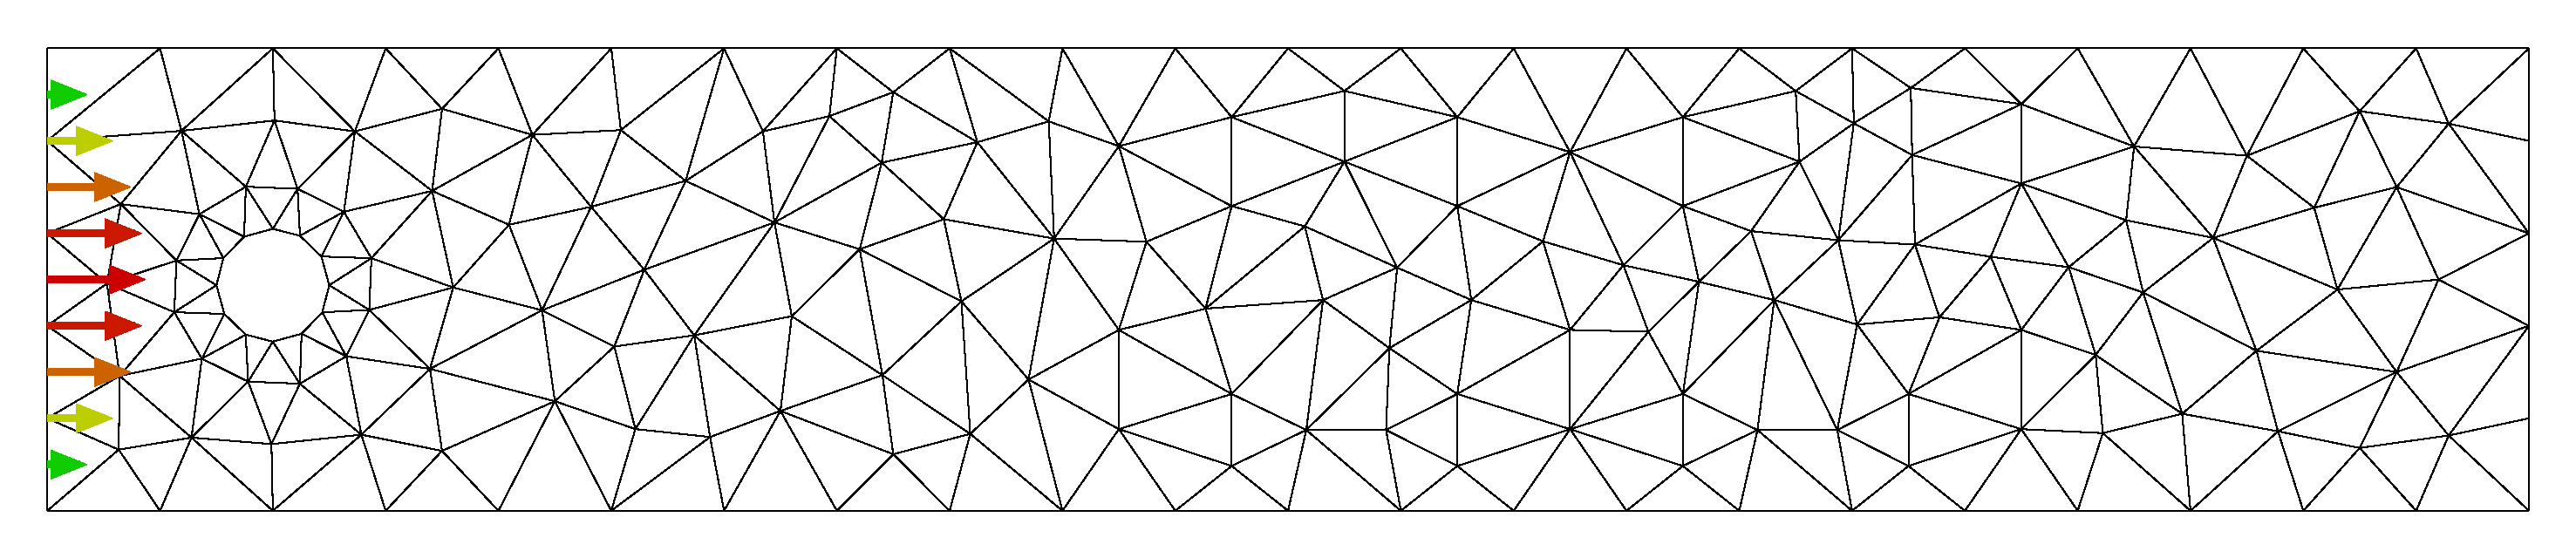
\includegraphics[width=\textwidth]{Figures/numerical_results/laminar_gpu/laminar_velocity_field_0.svg.pdf}
    		\caption{Laminar flow at t=0s}
    \end{subfigure}
\end{figure}

\begin{figure}[H]
	\ContinuedFloat
	\begin{subfigure}{\textwidth}
			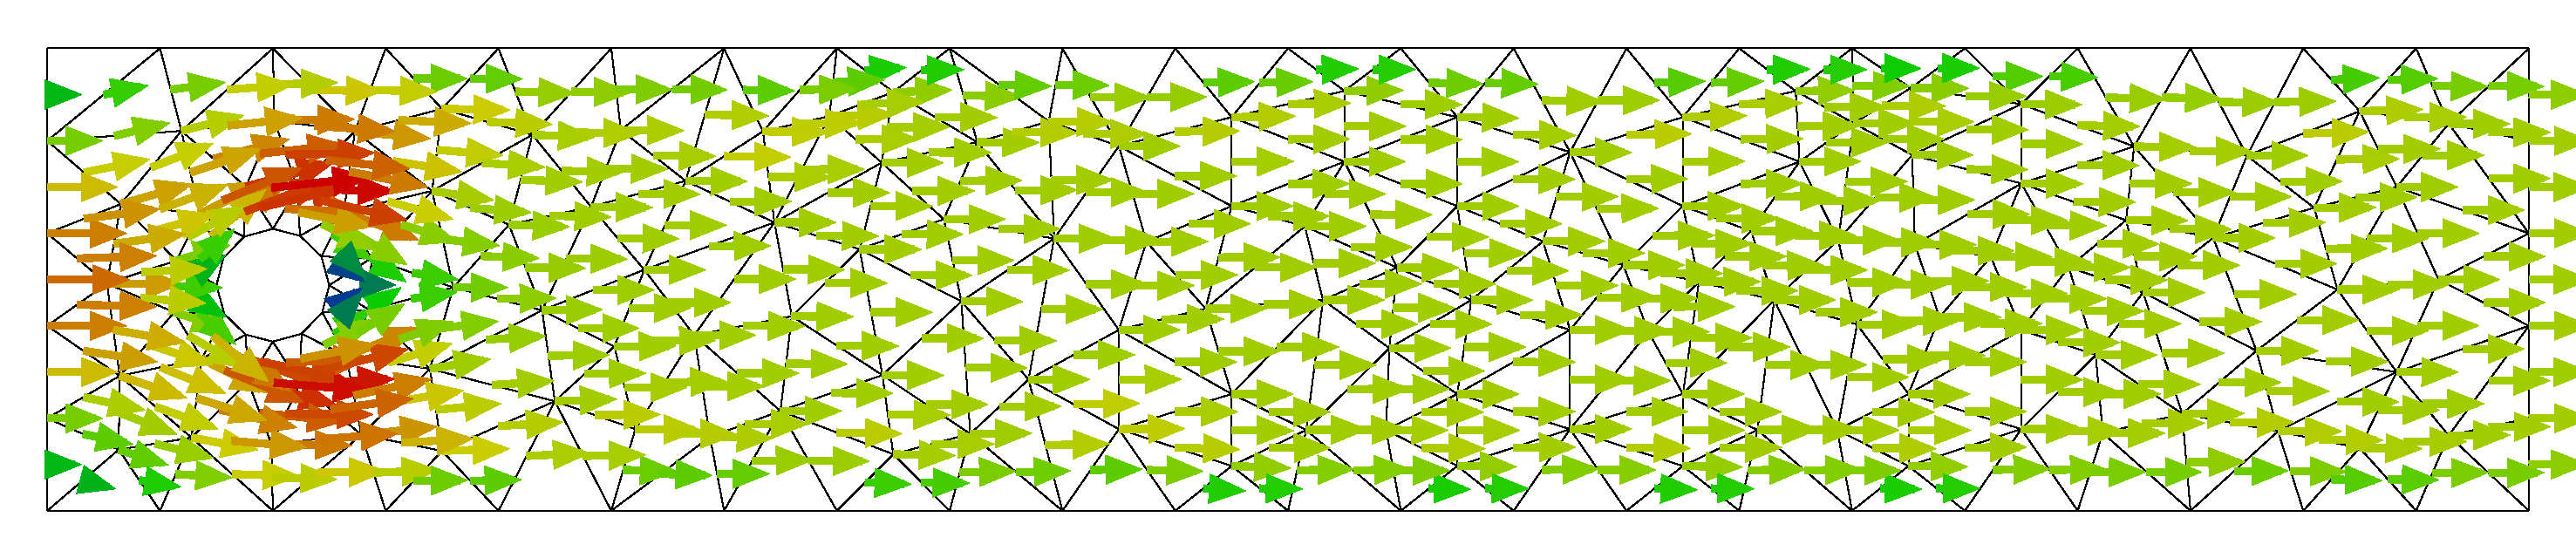
\includegraphics[width=\textwidth]{Figures/numerical_results/laminar_gpu/laminar_velocity_field_19.svg.pdf}
		\caption{Laminar flow at t=0.09s}
	\end{subfigure}
\end{figure}

\begin{figure}[H]
	\ContinuedFloat
	\begin{subfigure}{\textwidth}
    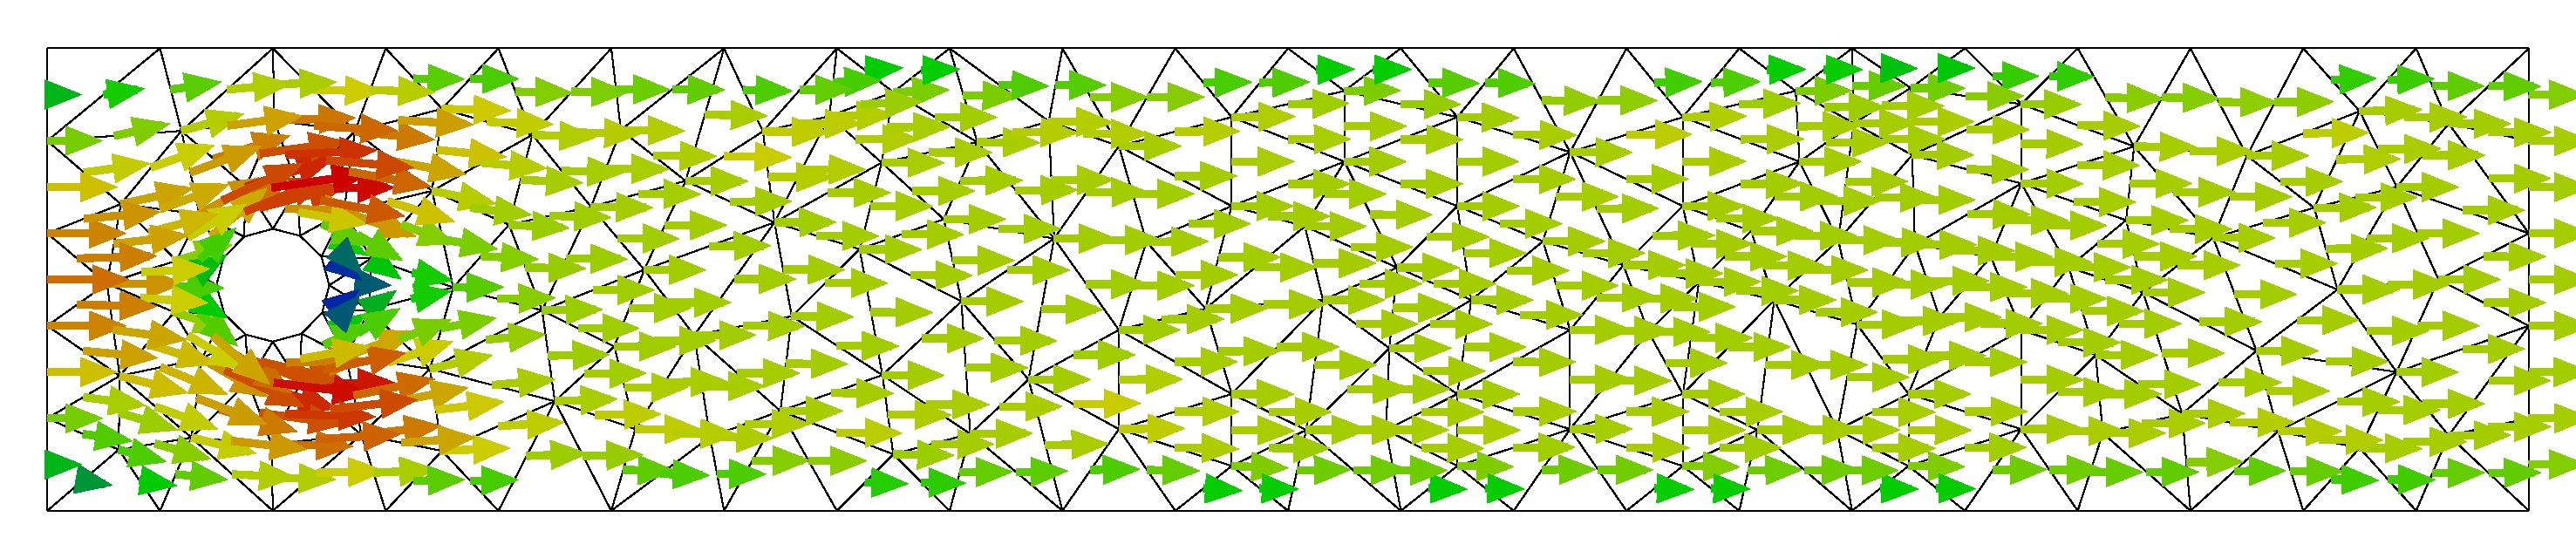
\includegraphics[width=\textwidth]{Figures/numerical_results/laminar_gpu/laminar_velocity_field_29.svg.pdf}
    \caption{Laminar flow at t=0.29s}
        \end{subfigure}
\end{figure}

\begin{figure}[H]
	\ContinuedFloat
	\begin{subfigure}{\textwidth}
    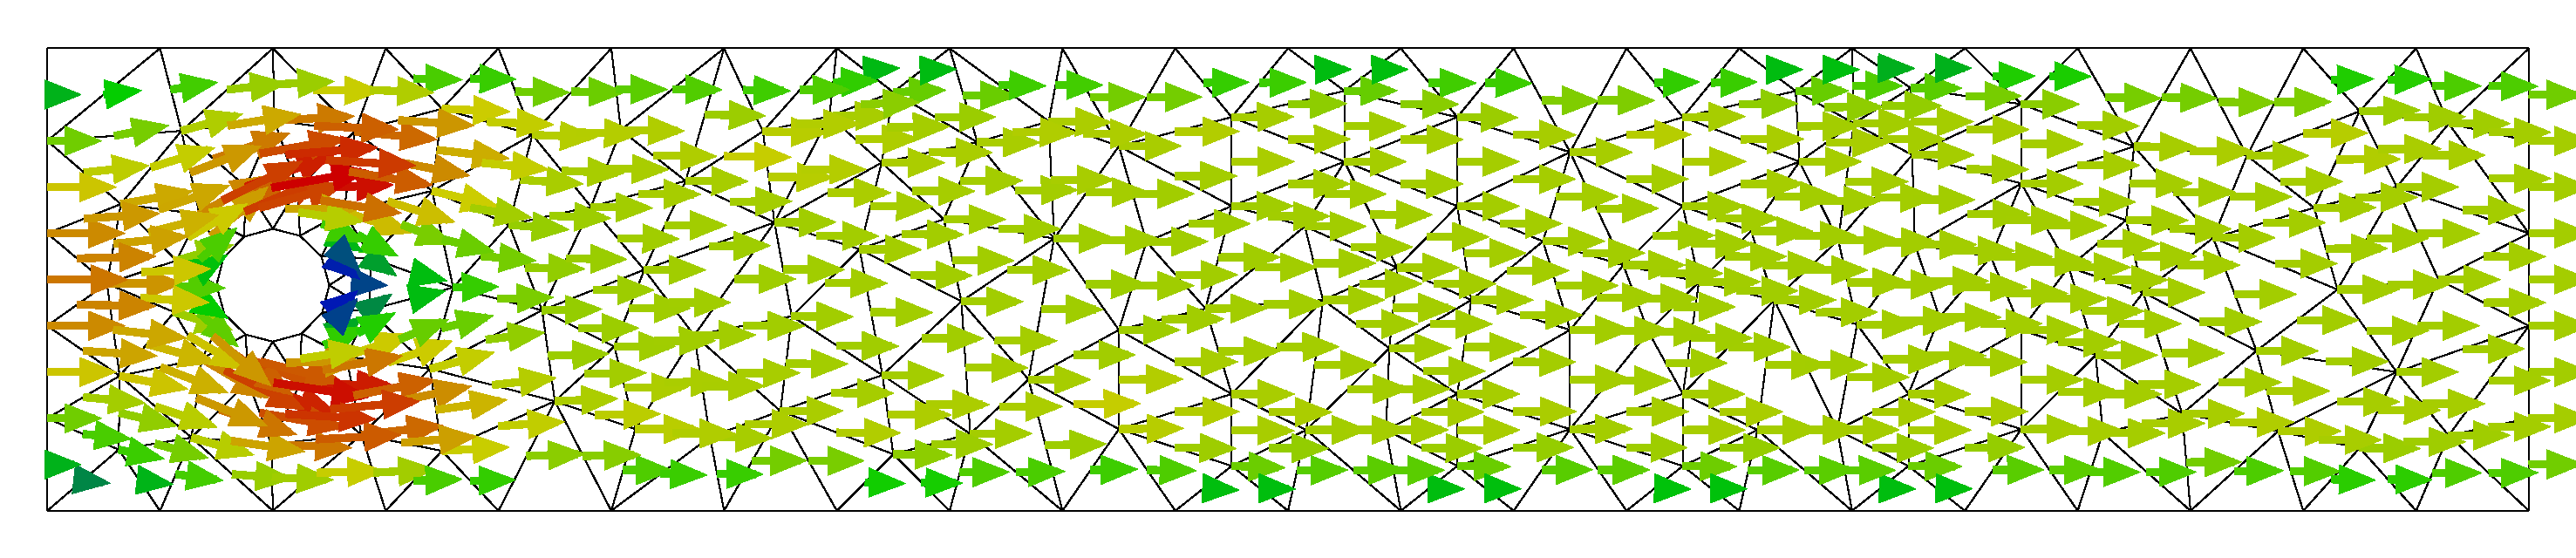
\includegraphics[width=\textwidth]{Figures/numerical_results/laminar_gpu/laminar_velocity_field_39.svg.pdf}
    \caption{Laminar flow at t=0.39s}
        \end{subfigure}
\end{figure}

\begin{figure}[H]
	\ContinuedFloat
	\begin{subfigure}{\textwidth}
    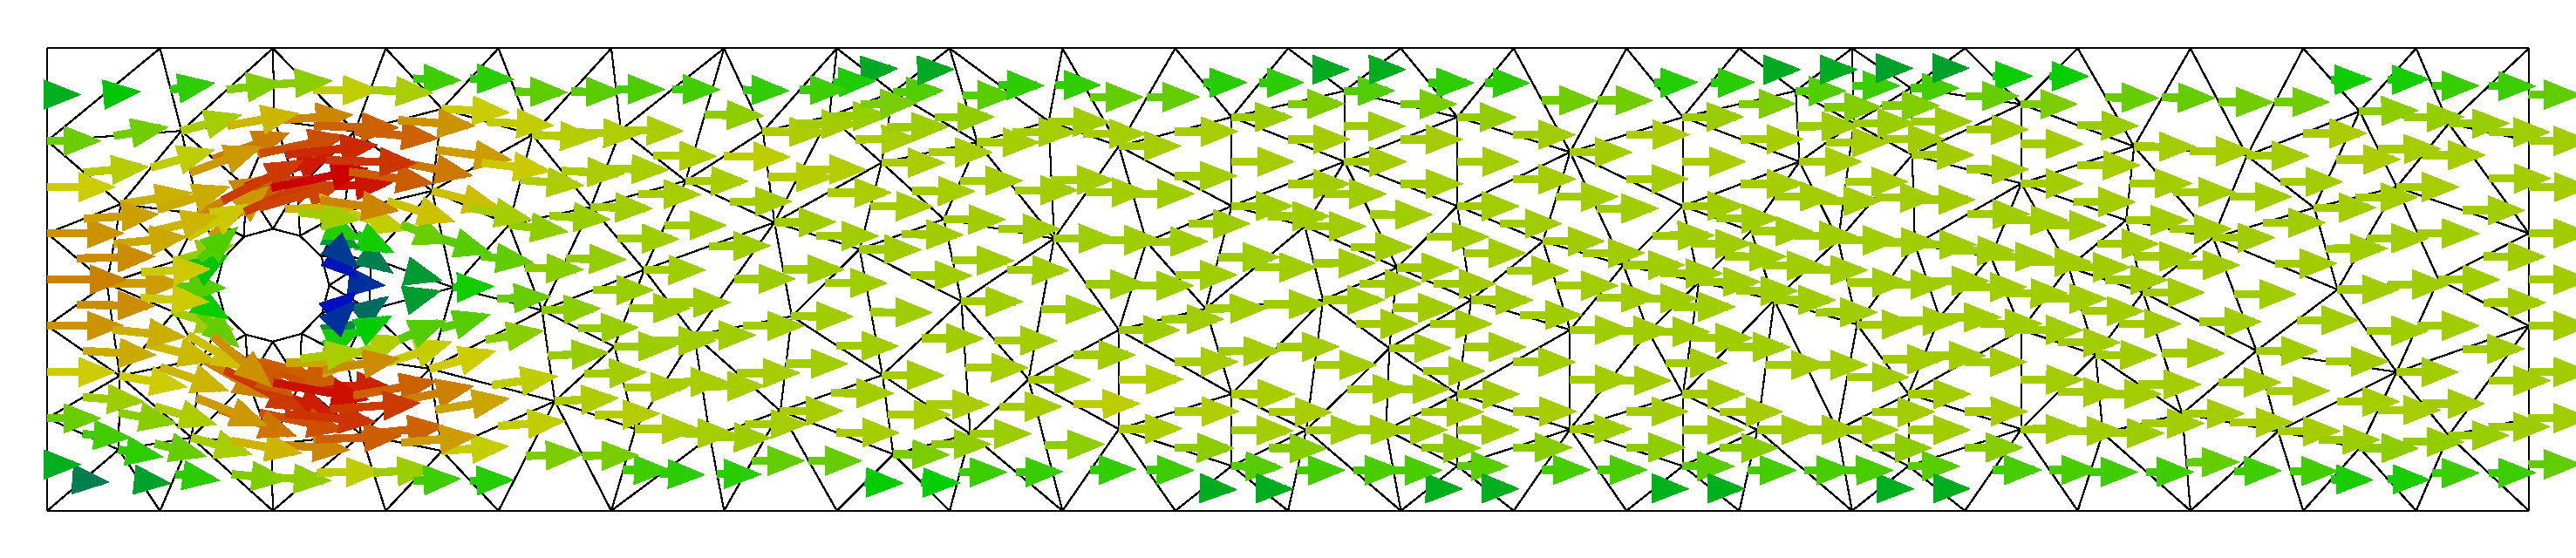
\includegraphics[width=\textwidth]{Figures/numerical_results/laminar_gpu/laminar_velocity_field_49.svg.pdf}
    \caption{Laminar flow at t=0.49s}
        \end{subfigure}
\end{figure}

\begin{figure}[H]
	\ContinuedFloat
	\begin{subfigure}{\textwidth}
    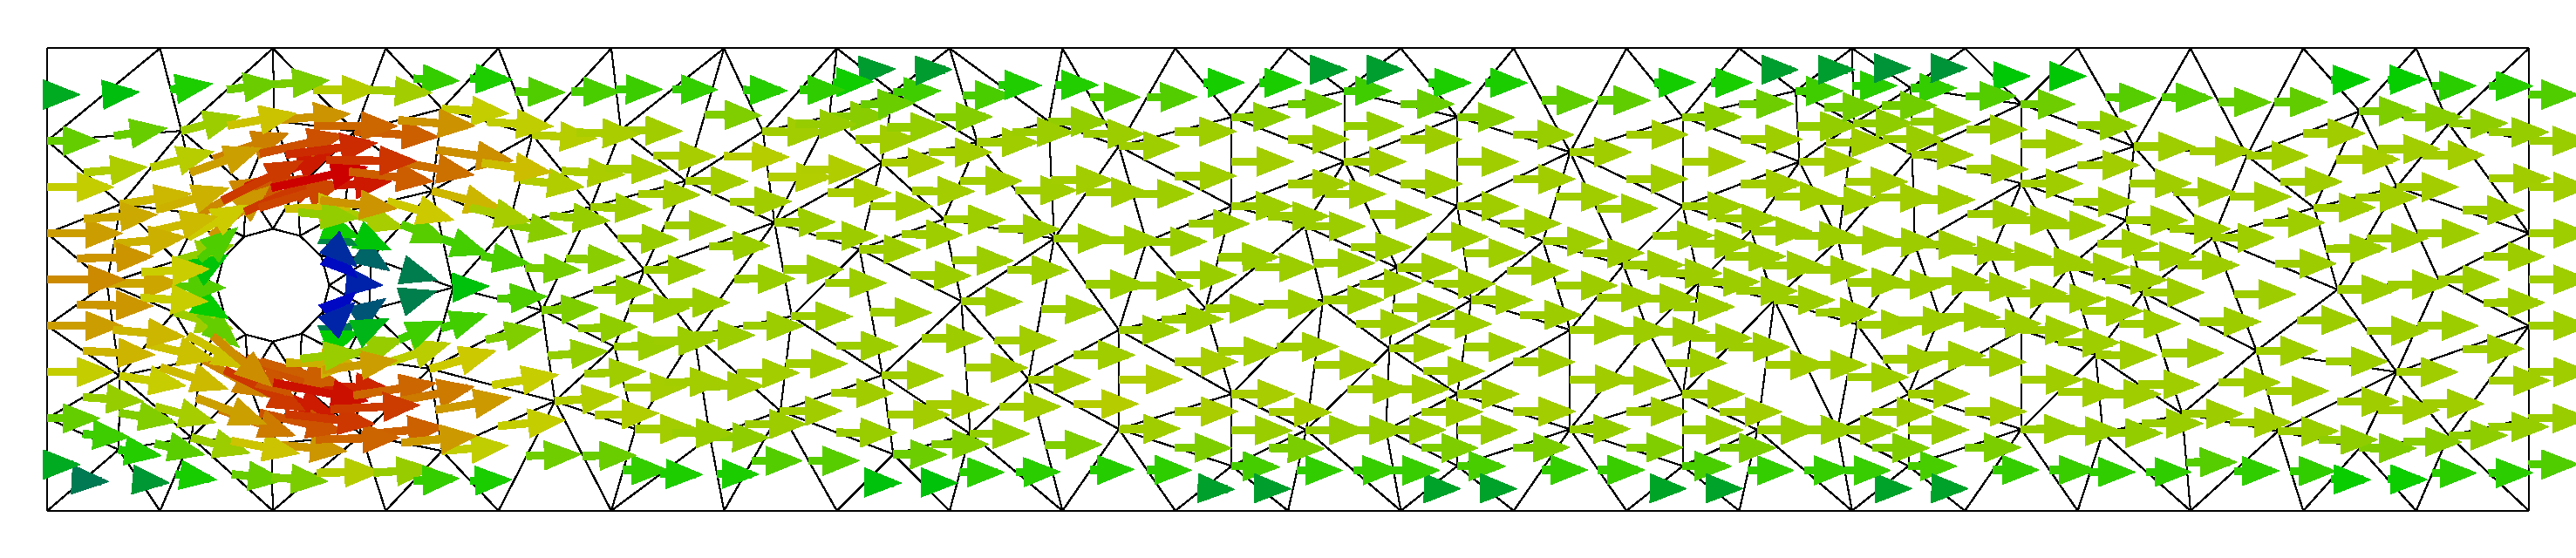
\includegraphics[width=\textwidth]{Figures/numerical_results/laminar_gpu/laminar_velocity_field_59.svg.pdf}
    \caption{Laminar flow at t=0.59s}
        \end{subfigure}
\end{figure}

\begin{figure}[H]
	\ContinuedFloat
	\begin{subfigure}{\textwidth}
    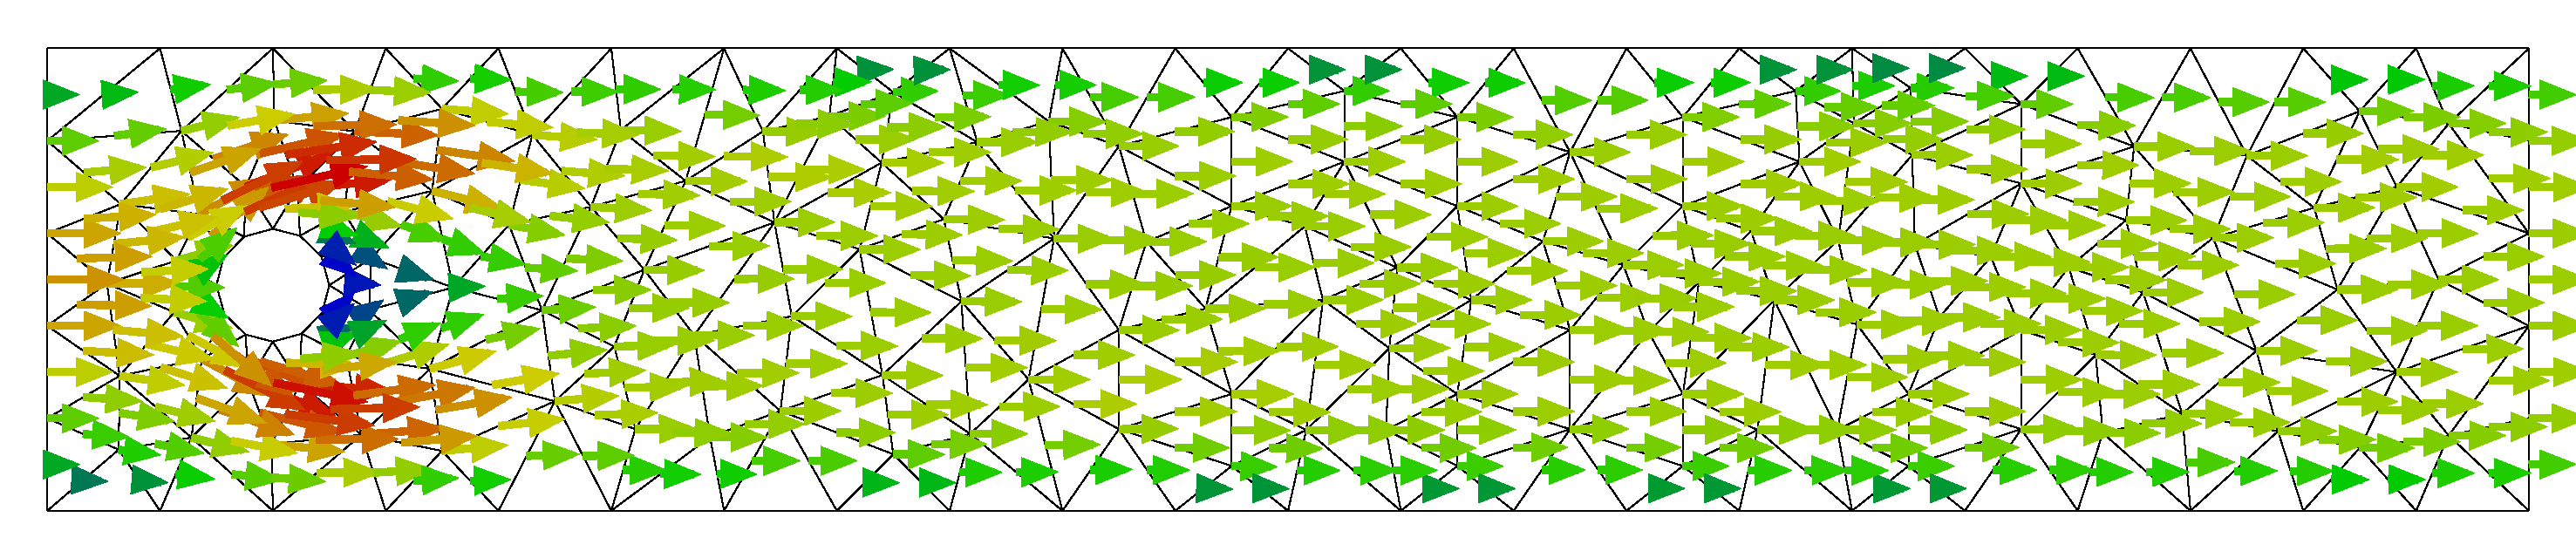
\includegraphics[width=\textwidth]{Figures/numerical_results/laminar_gpu/laminar_velocity_field_69.svg.pdf}
    \caption{Laminar flow at t=0.69s}
        \end{subfigure}
\end{figure}

\begin{figure}[H]
	\ContinuedFloat
	\begin{subfigure}{\textwidth}
    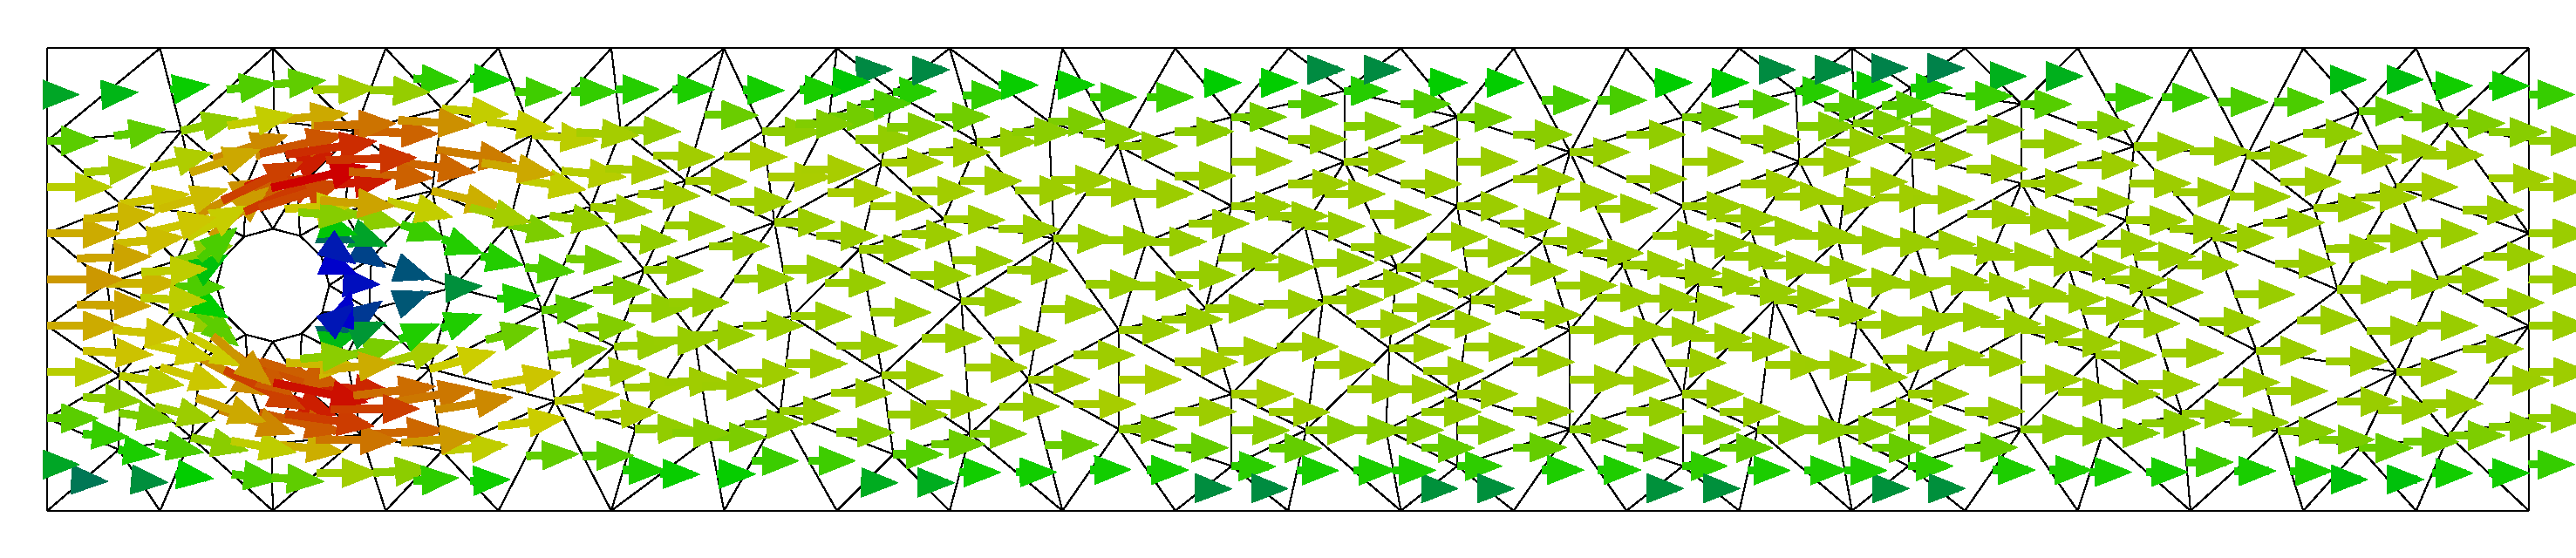
\includegraphics[width=\textwidth]{Figures/numerical_results/laminar_gpu/laminar_velocity_field_79.svg.pdf}
    \caption{Laminar flow at t=0.79s}
        \end{subfigure}
\end{figure}

\begin{figure}[H]
	\ContinuedFloat
	\begin{subfigure}{\textwidth}
    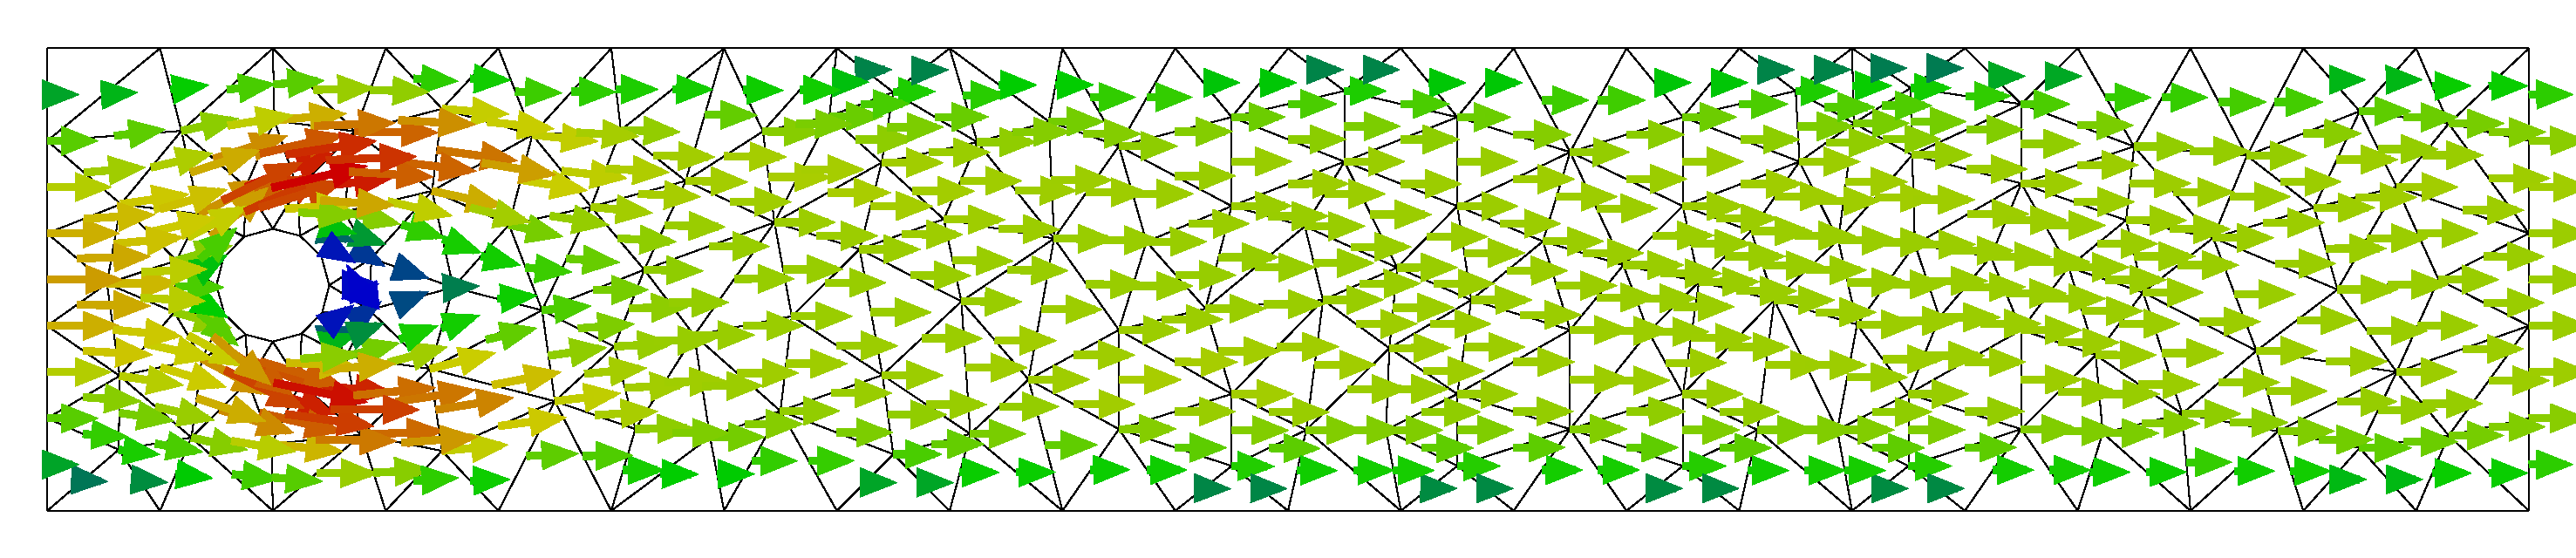
\includegraphics[width=\textwidth]{Figures/numerical_results/laminar_gpu/laminar_velocity_field_89.svg.pdf}
    \caption{Laminar flow at t=0.89s}
        \end{subfigure}
\end{figure}

\begin{figure}[H]
	\ContinuedFloat
	\begin{subfigure}{\textwidth}
    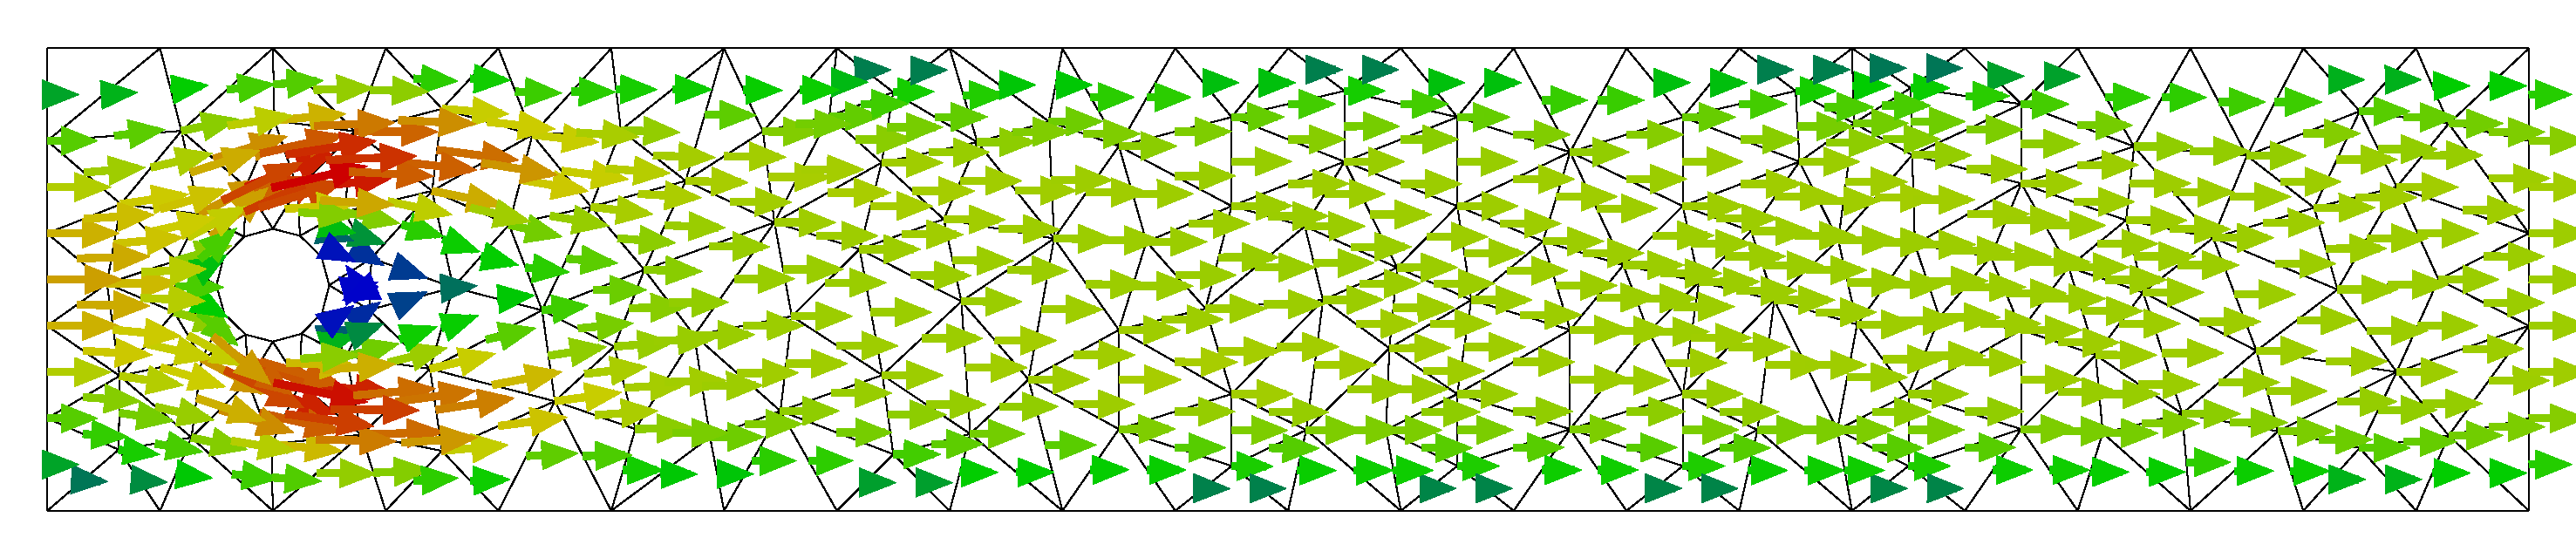
\includegraphics[width=\textwidth]{Figures/numerical_results/laminar_gpu/laminar_velocity_field_99.svg.pdf}
    \caption{Laminar flow at t=0.99s}
	\end{subfigure}
	\caption{Solution for laminar flow via \crefrange{eq:adv-diff-split-advect}{eq:adv-diff-split-diffuse} on GPU with $\Delta t = 0.01$.}
\end{figure}

\subsection{Turbulent Flow}
\begin{figure}[H]
	\centering
	\begin{subfigure}{\textwidth}
   	 	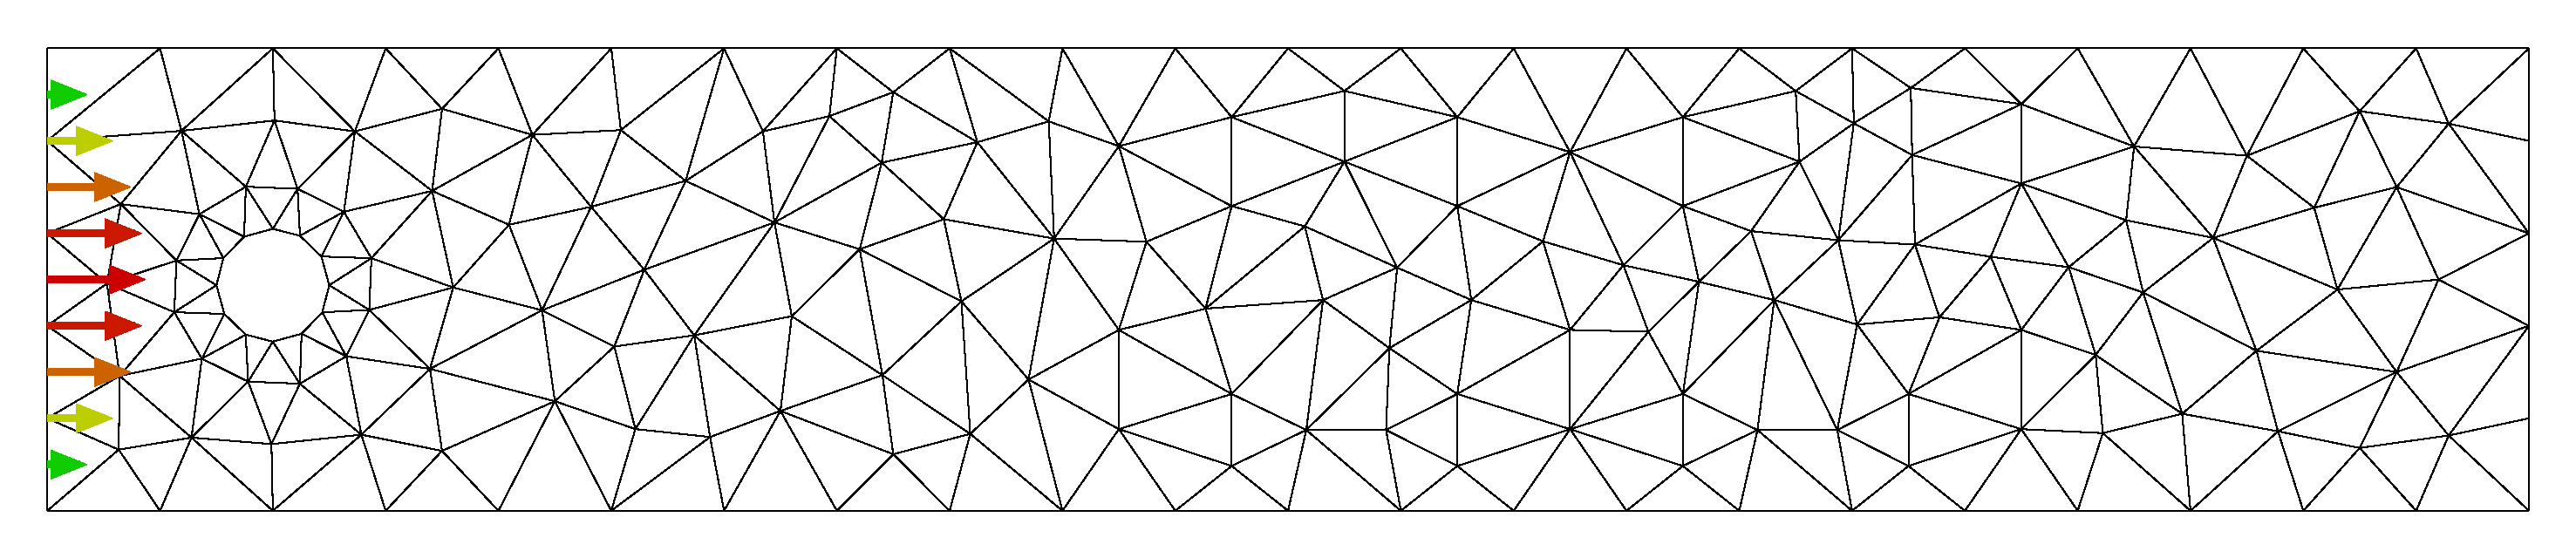
\includegraphics[width=\textwidth]{Figures/numerical_results/turbulent_gpu/turbulent_velocity_field_0.svg.pdf}
    		\caption{Turbulent flow at t=0s}
    \end{subfigure}
\end{figure}

\begin{figure}[H]
	\ContinuedFloat
	\begin{subfigure}{\textwidth}
    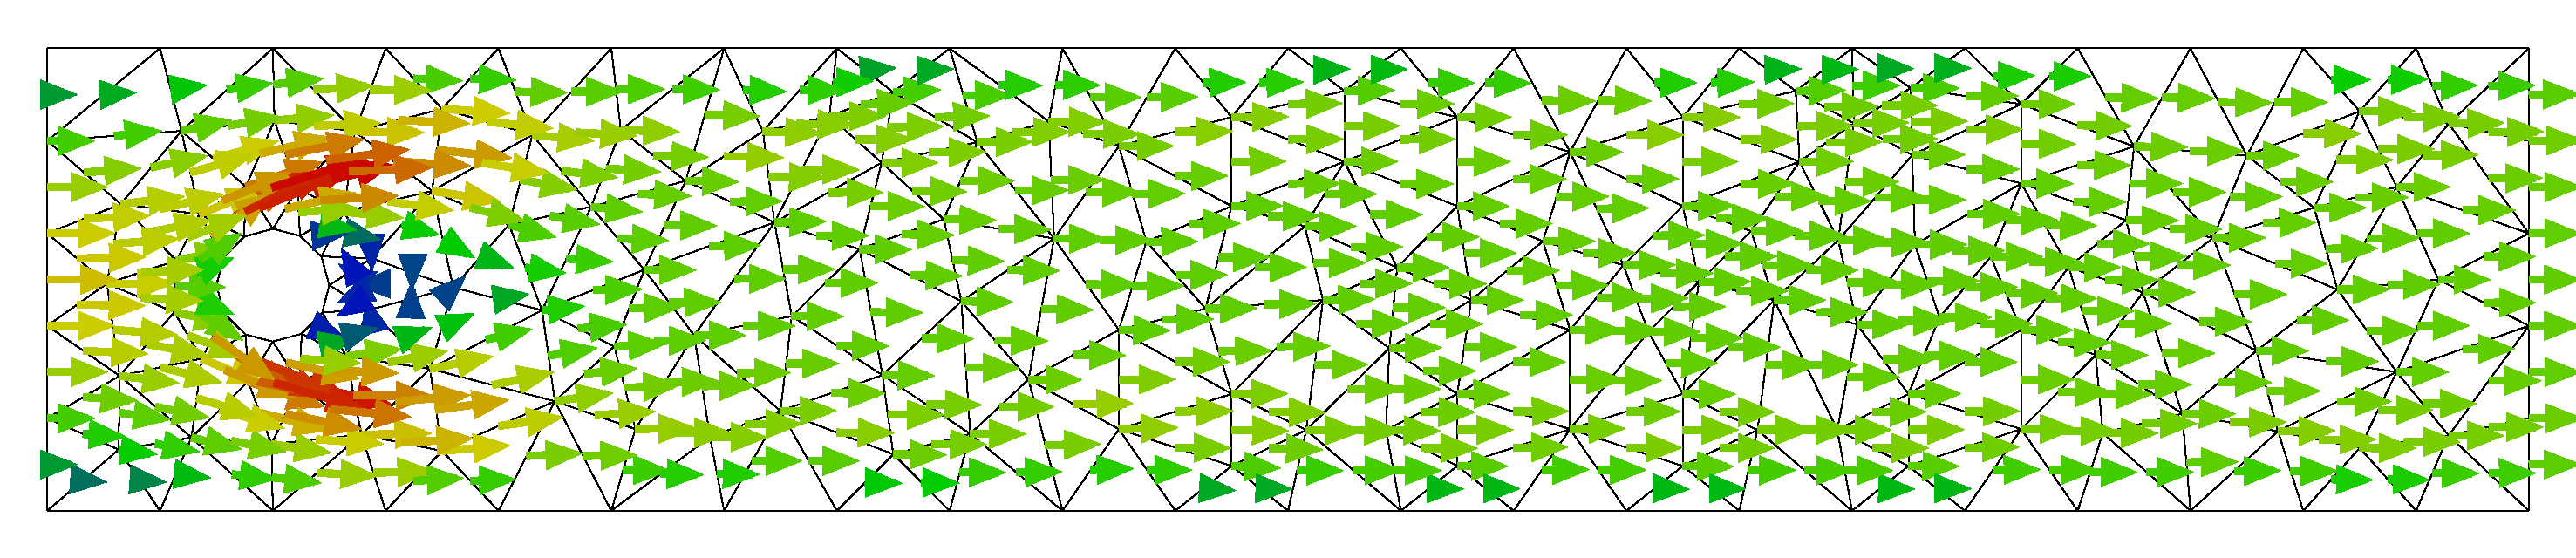
\includegraphics[width=\textwidth]{Figures/numerical_results/turbulent_gpu/turbulent_velocity_field_19.svg.pdf}
    \caption{Turbulent flow at t=0.09s}
        \end{subfigure}
\end{figure}

\begin{figure}[H]
	\ContinuedFloat
	\begin{subfigure}{\textwidth}
    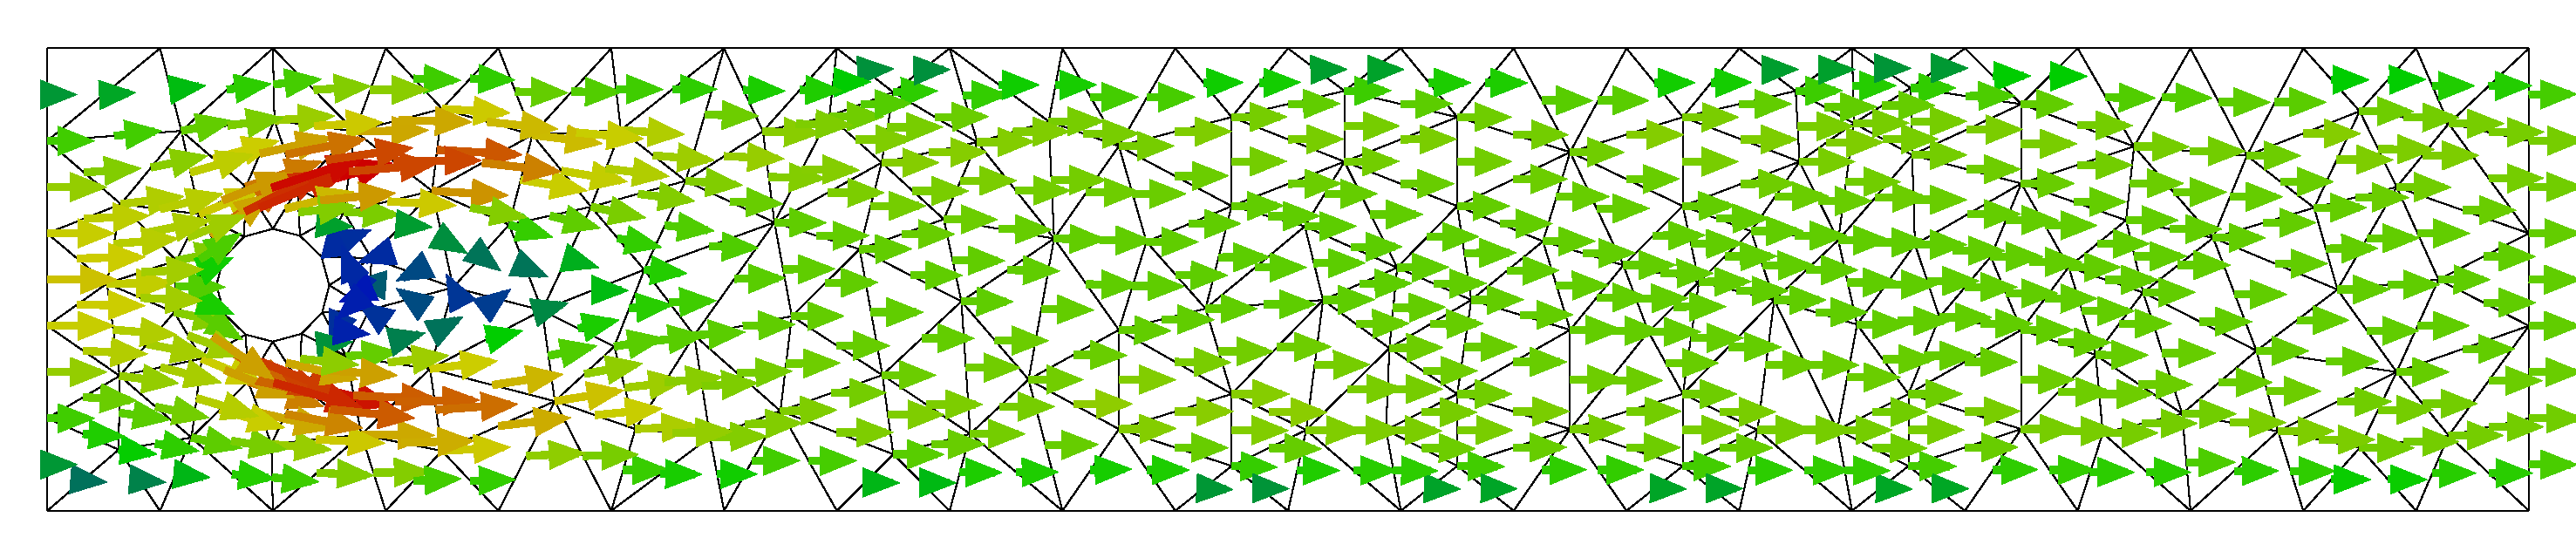
\includegraphics[width=\textwidth]{Figures/numerical_results/turbulent_gpu/turbulent_velocity_field_29.svg.pdf}
    \caption{Turbulent flow at t=0.29s}
        \end{subfigure}
\end{figure}

\begin{figure}[H]
	\ContinuedFloat
	\begin{subfigure}{\textwidth}
    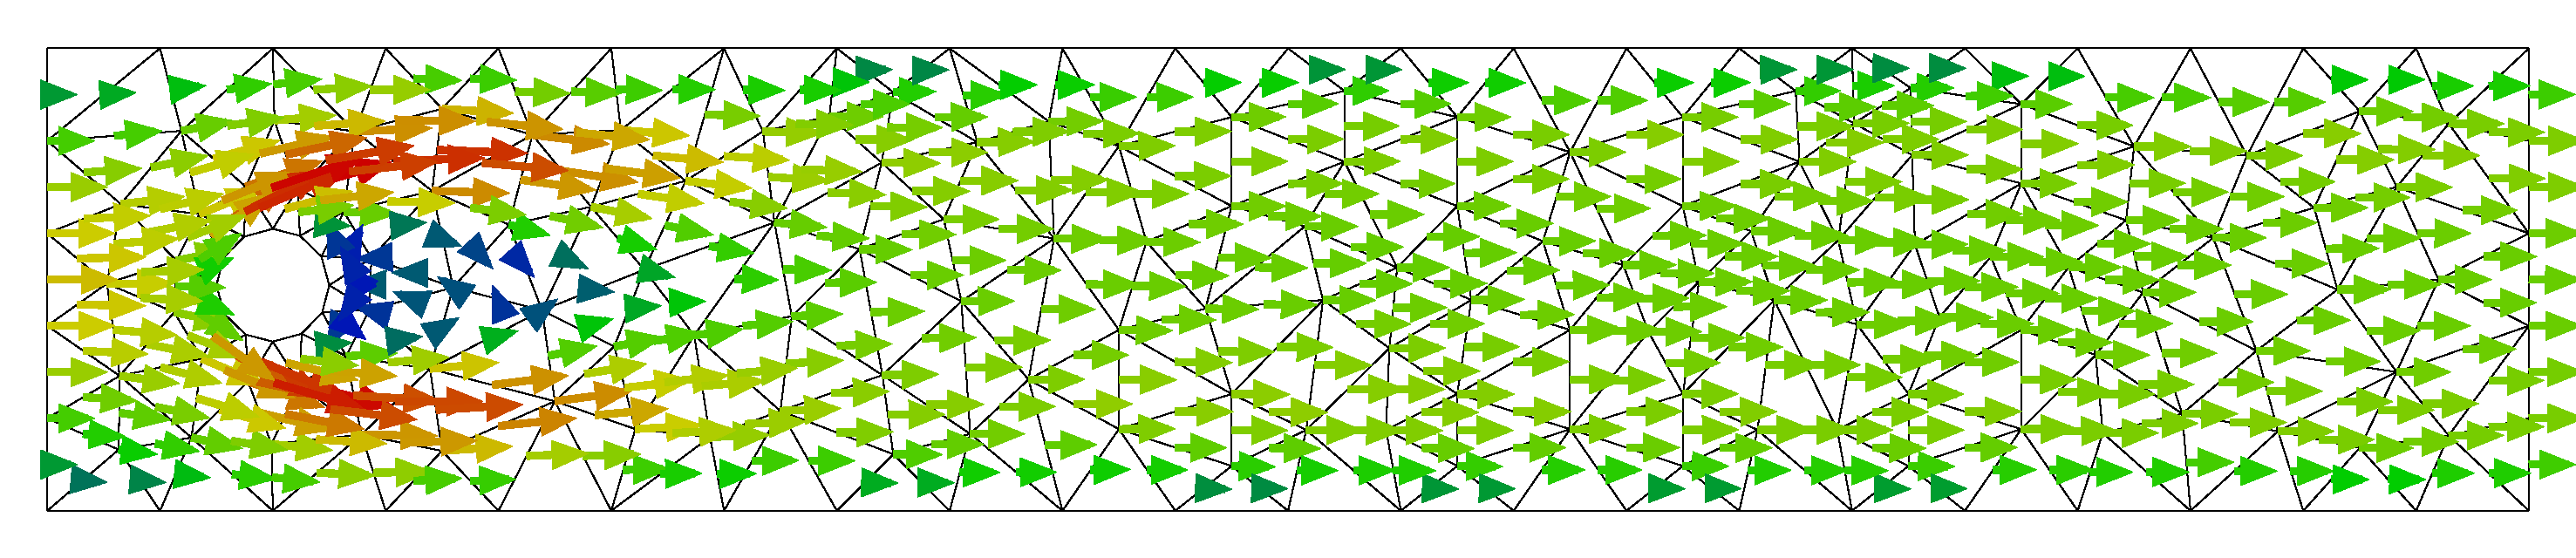
\includegraphics[width=\textwidth]{Figures/numerical_results/turbulent_gpu/turbulent_velocity_field_39.svg.pdf}
    \caption{Turbulent flow at t=0.39s}
        \end{subfigure}
\end{figure}

\begin{figure}[H]
	\ContinuedFloat
	\begin{subfigure}{\textwidth}
    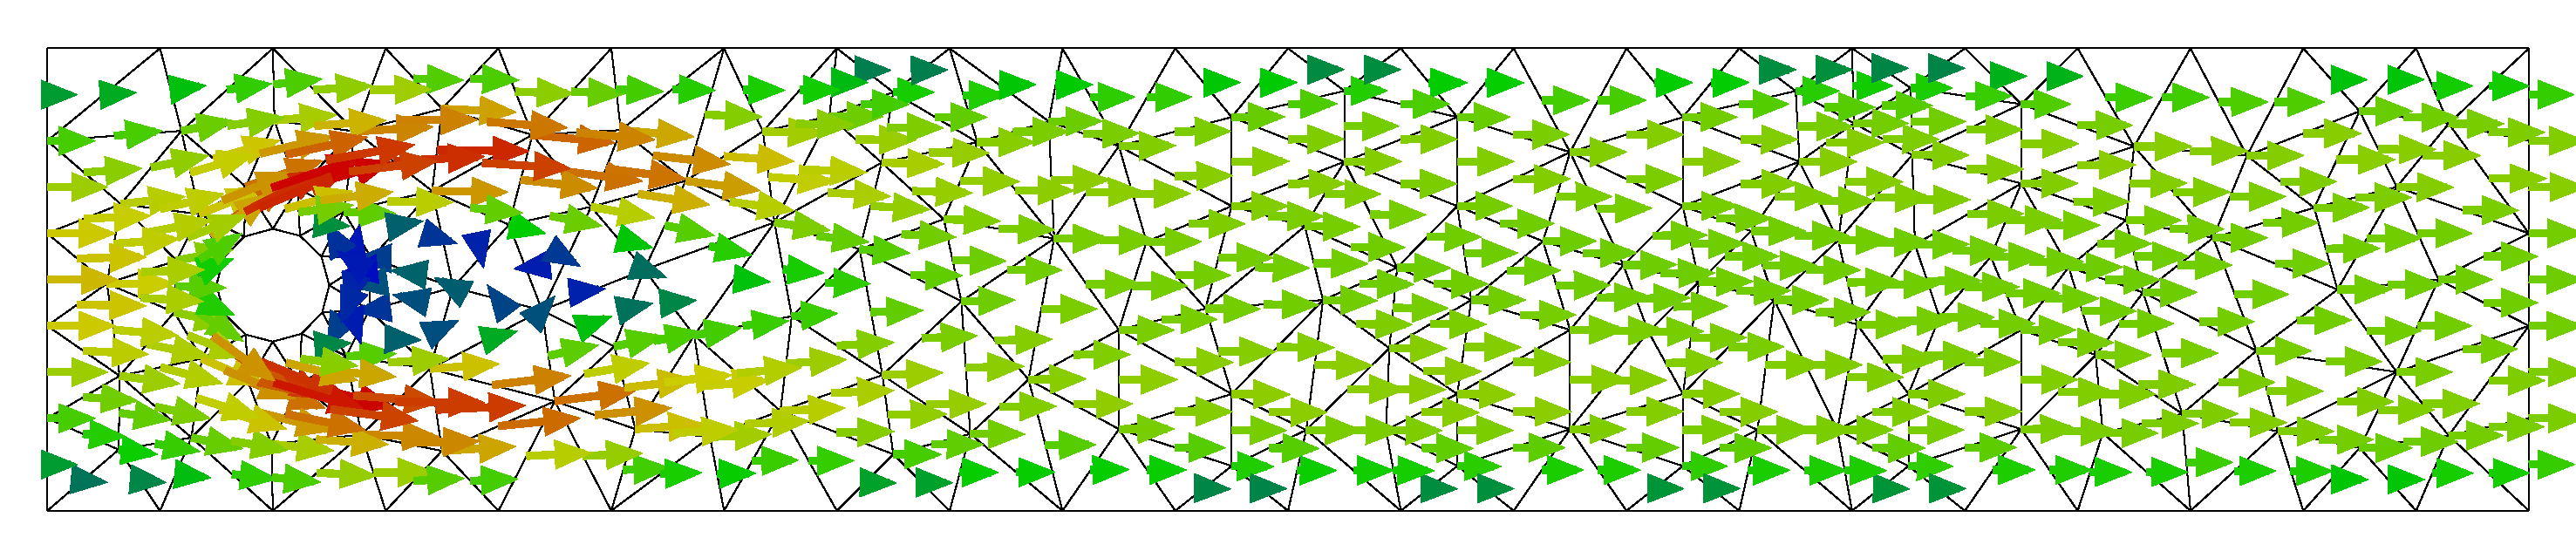
\includegraphics[width=\textwidth]{Figures/numerical_results/turbulent_gpu/turbulent_velocity_field_49.svg.pdf}
    \caption{Turbulent flow at t=0.49s}
        \end{subfigure}
\end{figure}

\begin{figure}[H]
	\ContinuedFloat
	\begin{subfigure}{\textwidth}
    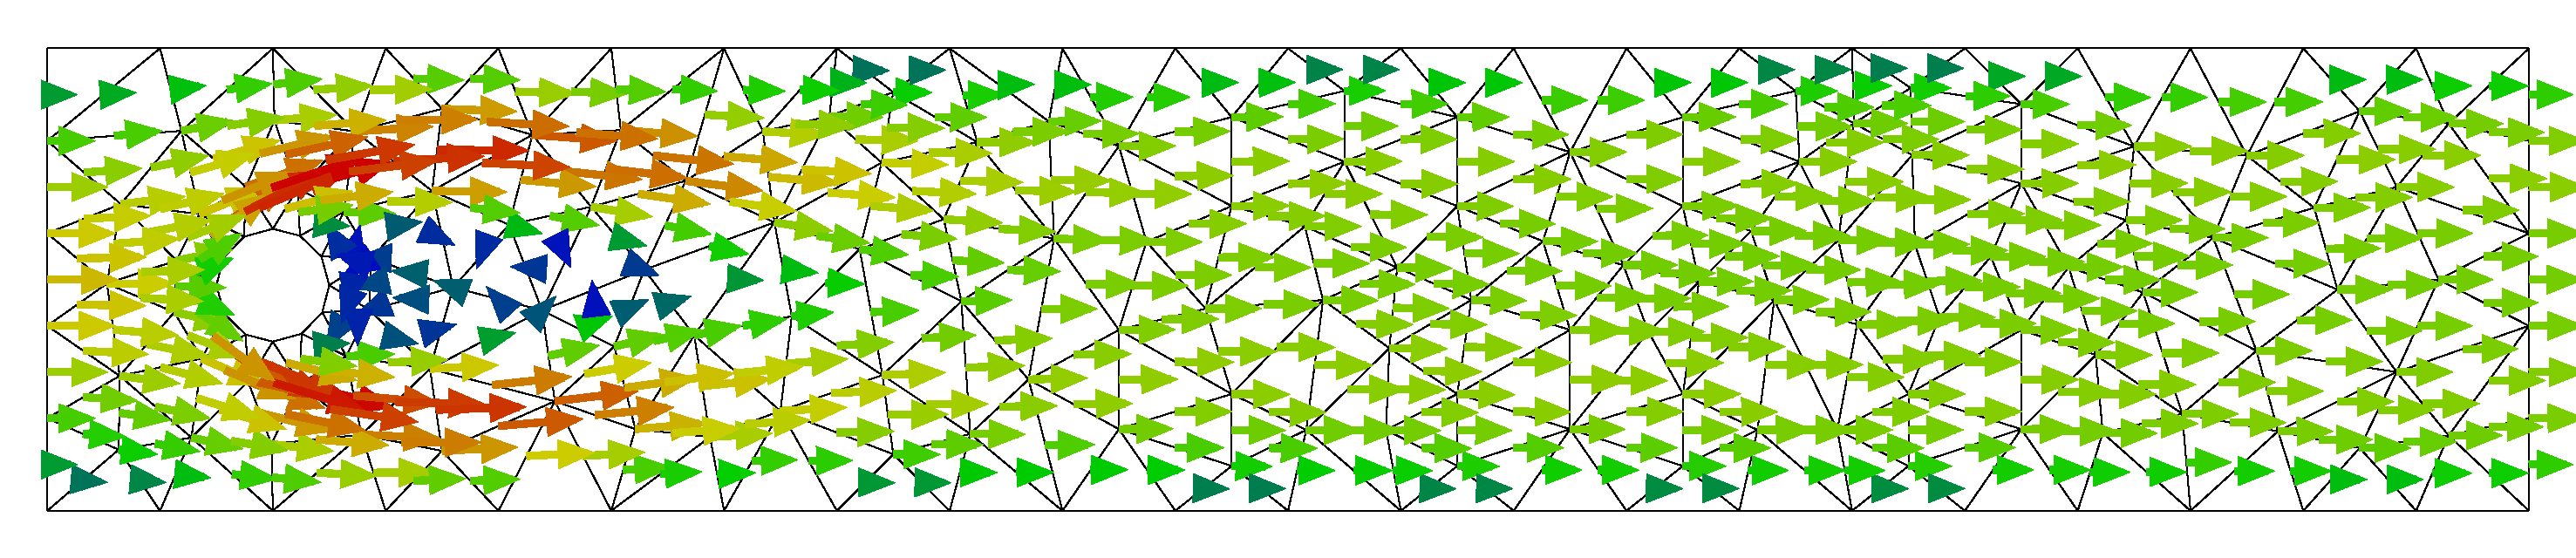
\includegraphics[width=\textwidth]{Figures/numerical_results/turbulent_gpu/turbulent_velocity_field_59.svg.pdf}
    \caption{Turbulent flow at t=0.59s}
        \end{subfigure}
\end{figure}

\begin{figure}[H]
	\ContinuedFloat
	\begin{subfigure}{\textwidth}
    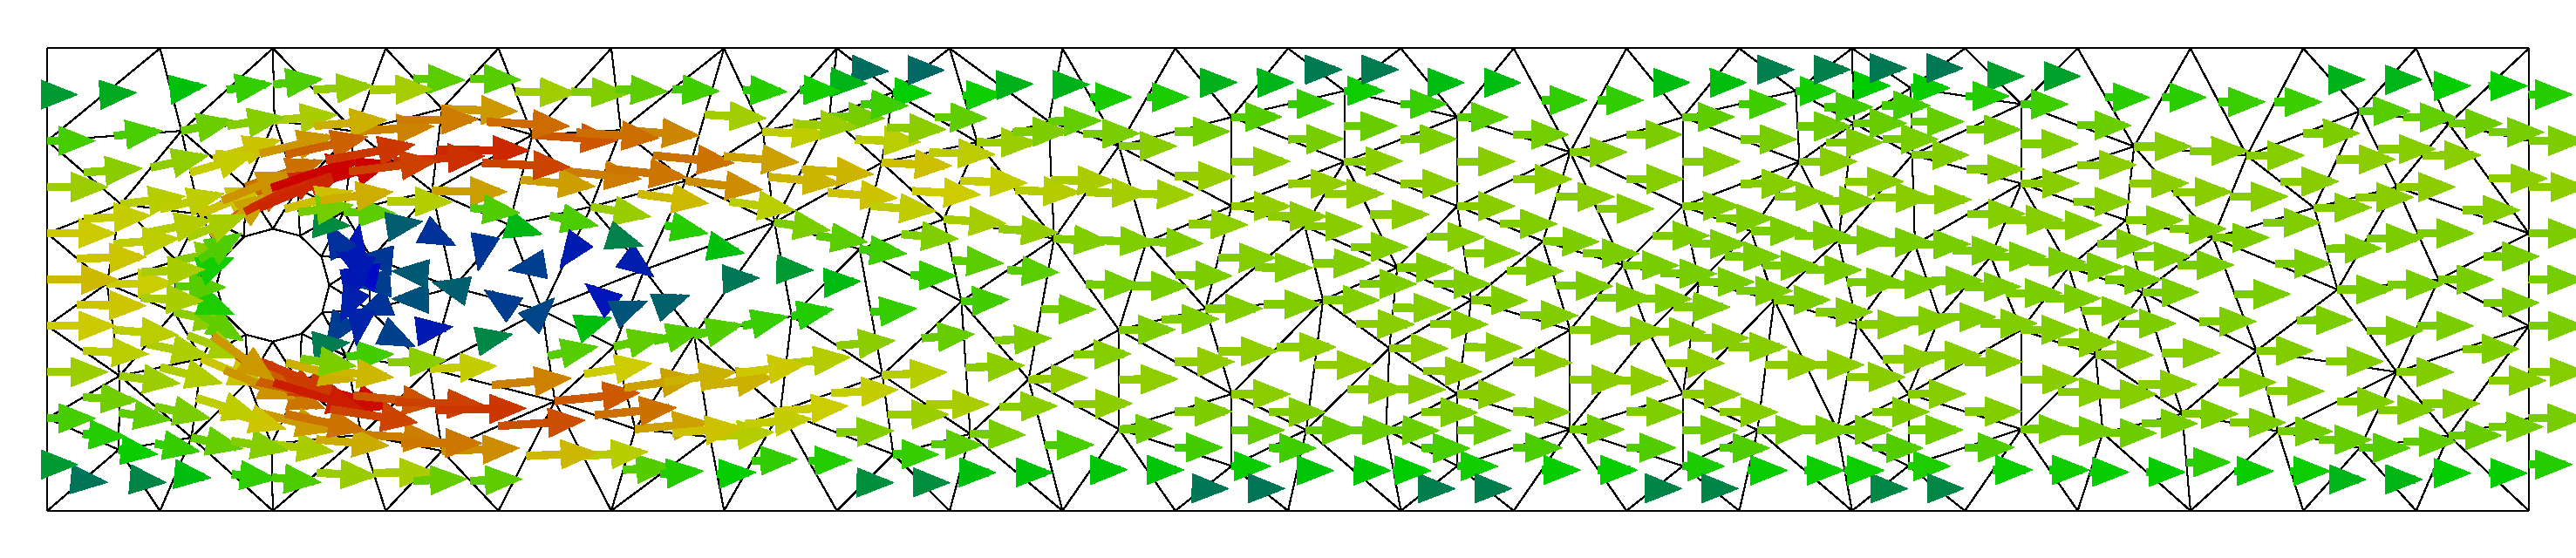
\includegraphics[width=\textwidth]{Figures/numerical_results/turbulent_gpu/turbulent_velocity_field_69.svg.pdf}
    \caption{Turbulent flow at t=0.69s}
        \end{subfigure}
\end{figure}

\begin{figure}[H]
	\ContinuedFloat
	\begin{subfigure}{\textwidth}
    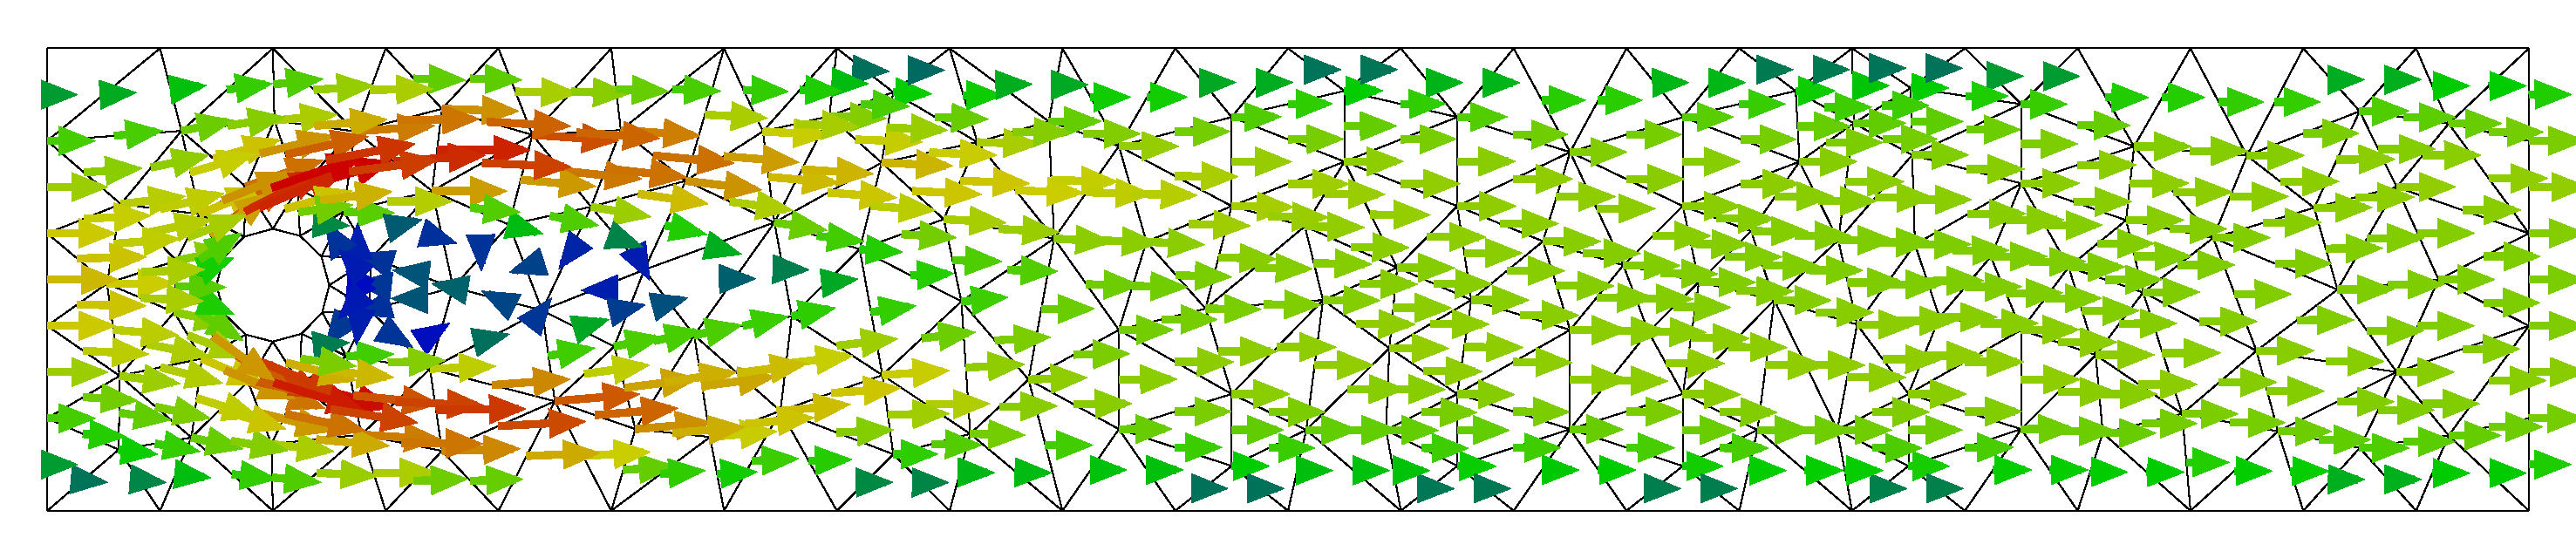
\includegraphics[width=\textwidth]{Figures/numerical_results/turbulent_gpu/turbulent_velocity_field_79.svg.pdf}
    \caption{Turbulent flow at t=0.79s}
        \end{subfigure}
\end{figure}

\begin{figure}[H]
	\ContinuedFloat
	\begin{subfigure}{\textwidth}
    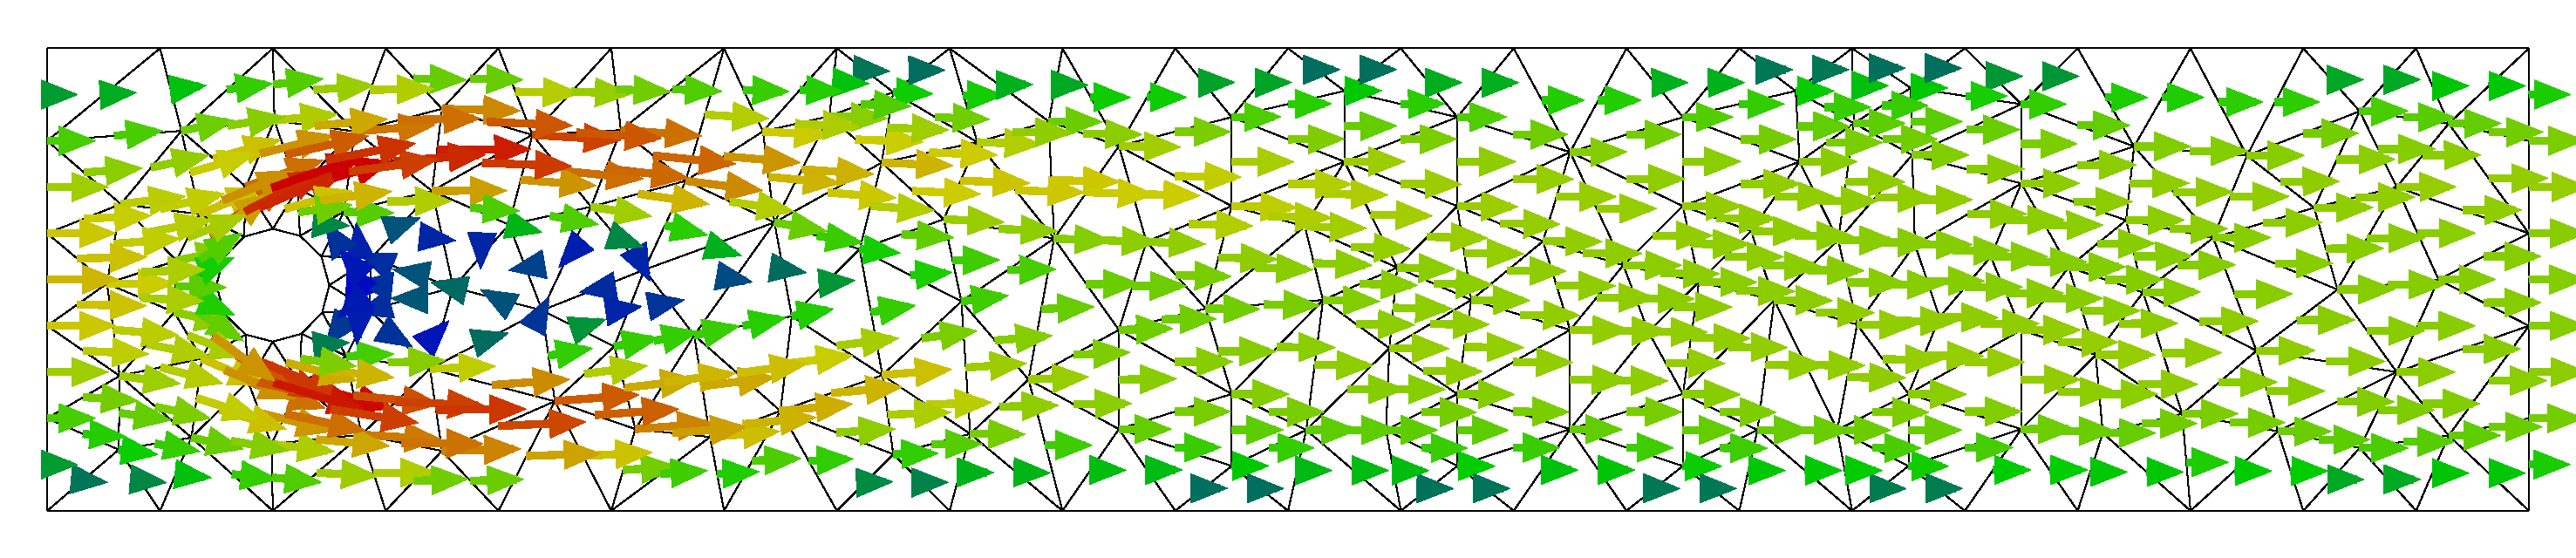
\includegraphics[width=\textwidth]{Figures/numerical_results/turbulent_gpu/turbulent_velocity_field_89.svg.pdf}
    \caption{Turbulent flow at t=0.89s}
        \end{subfigure}
\end{figure}

\begin{figure}[H]
	\ContinuedFloat
	\begin{subfigure}{\textwidth}
    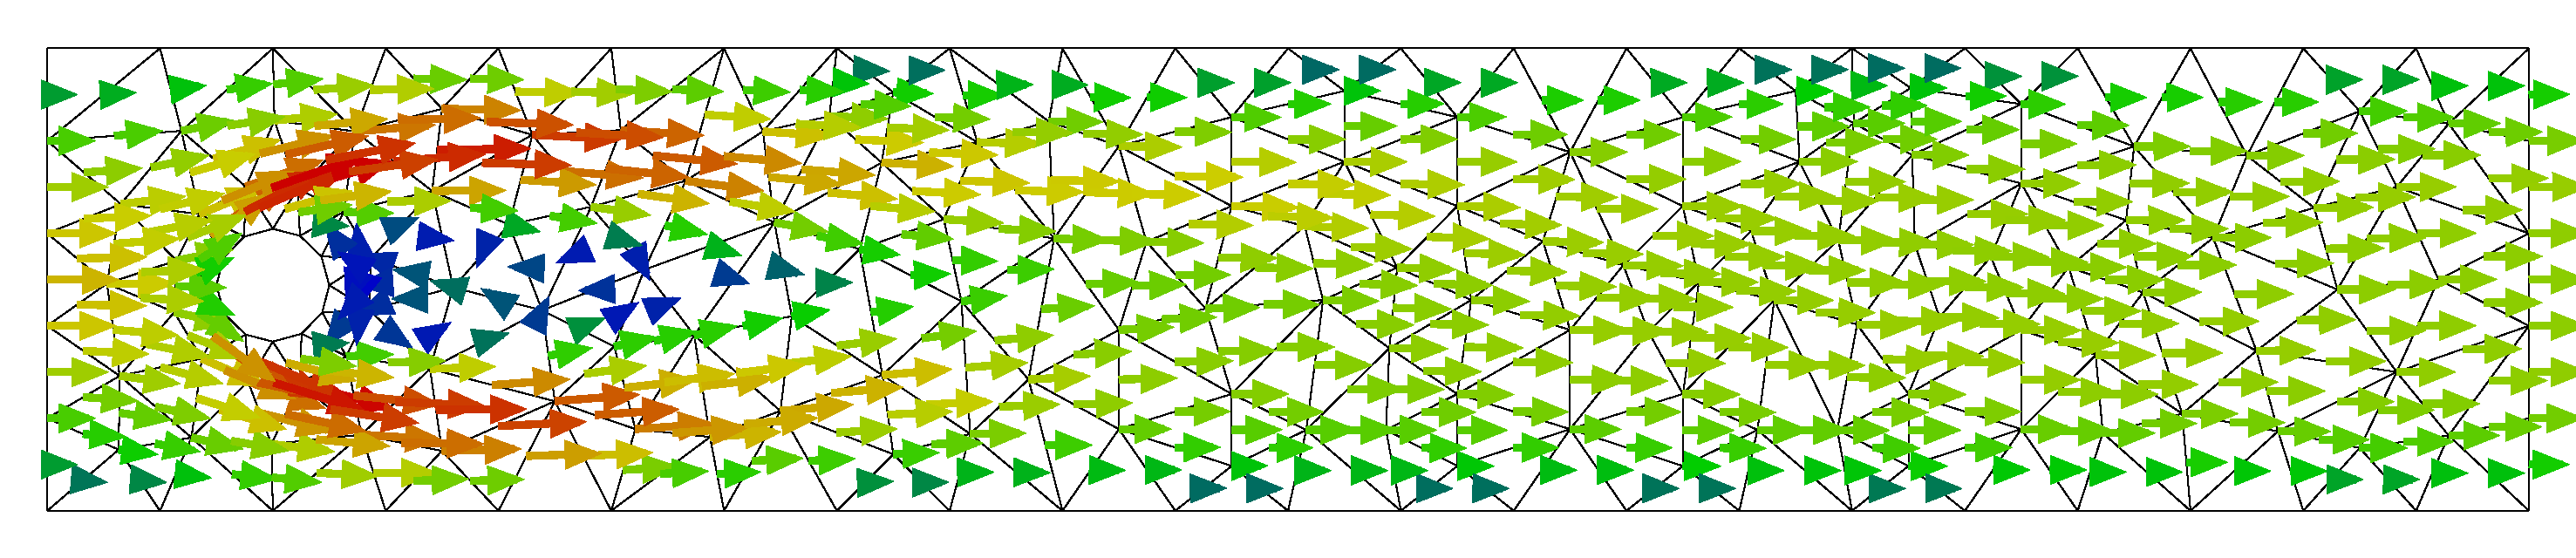
\includegraphics[width=\textwidth]{Figures/numerical_results/turbulent_gpu/turbulent_velocity_field_99.svg.pdf}
    \caption{Turbulent flow at t=0.99s}
	\end{subfigure}
	\caption{Solution for turbulent flow via \crefrange{eq:adv-diff-split-advect}{eq:adv-diff-split-diffuse} on GPU with $\Delta t = 0.01$.}
\end{figure}




\section{Comparison between GPU and CPU}
From the statistical data we can see that the GPU does better than the CPU. This, however, does not mean that CPUs are outdated. In general GPUs have less memory than a CPU and there is no way to add additional memory to a GPU. It is, also, hard to compare such vastly different hardware architectures. There are a lot of factors leading to the presented result. The GPU used in the numerical experiment is a rather high-end GPU, while the CPUs are mid/low end CPUs. More tests with different hardware, different problems and different meshes are needed in order to give a conclusive answer on which is better. This work, however, shows that there is potential in implementing GPU based FEM fluid solvers. As it was shown the GPU performs well when there are a lot of simple, independent computations. There are some opened questions however:
\begin{itemize}
	\item How suitable is the GPU for performing space discretization?
	\item How would the GPU perform in building the FEM matrices?
	\item How would the GPU perform in computing the IC0 preconditioner?
	\item How would the GPU perform in applying the IC0 preconditioner?
	\item How would the GPU perform in building the KD tree?
\end{itemize}
Most likely the GPU would not perform well in all of the above, thus a combination of CPU and GPU should be used.

\section{Further development}\label{ch:further-development}
Solving numerically the Navier-Stokes equations is a vast topic. We have not paid much attention to the type of the element we used. The $P_2P_1$ Taylor-Hood element is the simplest element which could be applied to this particular fractional time splitting algorithm. The semi-Lagrangian advection will fit nicely with quadrilateral elements in a structured grid. The accuracy and performance could be compared between the $P_2P_1$, $Q_2P^{-1}$ isoparametric element. It would be also interesting to compare the accuracy and performance when a divergence free element is used. The algorithm has to be tested in 3D, a good starting point would be the $Q_1Q_0$ element over a structured grid, which is very similar to the approach presented in \cite{Bridson}. The semi-Lagrangian method in 3D with unstructured meshes with tetrahedral elements, could become expensive due to the need to check whether a point lies in a tetrahedral. It should be evaluated if the algorithm is appropriate for such meshes.

The semi-Lagrangian method for unstructured meshes relies heavily on the efficient implementation of the KD Tree. We believe that the most important thing is to build a balanced KD Tree efficiently. The crucial part in building a balanced KD Tree is selecting the so-called splitting point. We have mentioned three possible ways to select the splitting point: using the PICK algorithm, Quickselect algorithm and using the approach presented in \cite{Balanced-KD-Tree}. The latter seems to be the most promising algorithm.

The implementation of the semi-Lagrangian advection allows the advection quantities to travel only in straight lines, a multi staged semi-Lagrangian method could be implemented. This will allow the imaginary particles to have curved trajectories, which is more realistic. A good start would be \cite{Fract-Seim-Lag}.

It was noted that multithreading the assembling of the matrices in a sparse (CSR) format is not trivial and relies on graph coloring. It is worth trying to implement it, however. It has two advantages. First it could speed up the assembly phase. Second when such an algorithm is implemented the advection phase could be solved using the FEM and compared to the semi-Lagrangian method.

The performance of the CPU implementation of the CG and PCG methods will be improved if SIMD instructions are used. The computation and application of the IC0 preconditioner must be multithreaded. A good starting point for a GPU implementation would be \cite{MT-PCG-NV}. Multithreaded Block Jacobi preconditioner should be implemented and compared to the multithreaded IC0 preconditioner.

Different algorithms, e.g. Runge-Kutta, can be used to improve the accuracy of the approximation of the time derivatives. However, it can be shown \cite{Bridson} that the splitting technique which was used provides $O(\Delta t)$ accuracy. This means a higher order splitting technique is required. For example the Strang splitting could be used.

\chapter*{Conclusion} 
\addcontentsline{toc}{chapter}{Conclusion}
Over the course of this work 3 different algorithms for solving the Navier-Stokes equations. One of them matched our goals (performance, scalability and accuracy) and was further developed both on CPU and GPU. The algorithm splits the differential operator into three parts: advection, diffusion and pressure projection. Semi-Lagrangian method accelerated by KD Tree data structure was presented for the advection part and it was shown that it scales well both on CPU and GPU. Both the diffusion and the pressure projection parts boil down to solving linear systems with SPD matrices. The CG method was used for solving the systems. For the GPU implementation two implementations were presented: a multi kernel and a mega kernel. It was shown that the mega kernel is about four times faster than the multi kernel implementation. Although the implementation of the mega kernel CG was  trivial, we could not find another resource which presents it, nor a resource which provides comparison between the two approaches. The PCG method, using IC0 preconditioner, was also implemented and it was shown that it reduces the number of iterations about two times. Our implementation of the PCG method did not use multiple threads applying the preconditioner (line \ref{alg-line:apply-preconditioner} of \cref{alg:pcg}) and thus performed worse than the CG method, despite the smaller number of iterations.